\documentclass[11pt]{article}

\usepackage[margin=1in]{geometry}
\usepackage{amsmath}
% Times text and mathematics, matching the manuscript and the journal's font
% instruction; and the journal's small, non-italicized p for p-values.
\usepackage{newtxtext,newtxmath}
\newcommand{\pval}{\mathrm{p}}
% Line numbers on the review copy, as on the manuscript, so referees can
% point at supplement lines too.
\ifdefined\journalreviewcopy
  \usepackage[right]{lineno}
\fi
\usepackage{array,booktabs,longtable,multirow}
\usepackage{cite}
\usepackage{graphicx}
\usepackage{hyperref}
\usepackage{microtype}
\usepackage{pdflscape}
\usepackage{setspace}
\usepackage[labelfont=bf,labelsep=period,justification=raggedright,singlelinecheck=false]{caption}
\hypersetup{hidelinks}
\bibliographystyle{vancouver}
\doublespacing

\title{Supplementary material for\\
\large Playing time tracks recent exposure in fifteen men's and women's football leagues: the denominator gradient and what it does to per-minute injury rates}
% The supplement travels to referees, so it blinds the same way the
% manuscript does: author identity lives only in the separate title page.
\ifdefined\journalblindcopy
  \author{}
\else
  \author{Gustavo Pedro Ricou and Nicholas Mahony}
\fi
\date{}

\begin{document}
\ifdefined\journalreviewcopy
  \linenumbers
\fi
\maketitle

This supplement contains the analyses that support, but do not compete with, the main measurement-sensitivity results. Supplementary Data S1 is \path{jsams_revised_hypothesis_register.csv}. It contains 706 unique rows: the 637 legacy exploratory tests plus all 63 exposure-multiverse tests, three temporal slopes, one temporal-heterogeneity test and two conditional estimates. Each row gives its model, contrast, target outcome, denominator, raw value, multiplicity family, adjusted value, analysis timing and estimable status. No analysis was pre-specified or confirmatory.

\section{STROBE checklist}

Table~\ref{tab:supp_strobe} is the completed STROBE checklist for cohort studies \cite{vonelm2007strobe}, read together with the consensus statement on injury-surveillance reporting in football \cite{bahr2020ioc}. It is generated rather than typed. Every row names one or more locations in the manuscript, those locations are looked up in the manuscript source when the table is built, and a row pointing at a heading that has since been renamed or cut stops the build instead of reaching a reader as a false statement. The resolution is deposited alongside the table, so the checking can be inspected rather than taken on trust.

Two entries are worth reading as substantive rather than procedural. Item~12d has no analogue here: the design follows appearances, not individuals through follow-up, so there is no loss to follow-up to address, and the checklist says so instead of leaving the row blank. Item~3 records that no hypothesis was prespecified; the manuscript states this in the same words, and the reference association is labelled a worked example wherever it appears.

% Generated by src/43_strobe_checklist.py. Do not edit by hand: every
% anchor here was resolved against manuscript.tex when this was written,
% and editing the table breaks that guarantee silently.
\begingroup
\footnotesize
\setlength{\LTcapwidth}{\textwidth}
\begin{longtable}{@{}p{0.05\textwidth}p{0.30\textwidth}p{0.57\textwidth}@{}}
\caption{STROBE checklist for cohort studies, completed for this manuscript. Each item names the location in the manuscript that addresses it; the locations are resolved against the manuscript source by \texttt{src/43\_strobe\_checklist.py}, which fails rather than emit an item pointing at text that is not there.}\label{tab:supp_strobe}\\
\toprule
Item & Recommendation & Where addressed \\
\midrule
\endfirsthead
\toprule
Item & Recommendation & Where addressed \\
\midrule
\endhead
\bottomrule
\endfoot
1a & Indicate the study's design with a commonly used term in the title or the abstract & The abstract opens the methods sentence with the design term. The title names the populations and the measurement rather than the design, so the abstract carries item 1a. \\
\addlinespace[2pt]
1b & Provide in the abstract an informative and balanced summary of what was done and what was found & The unstructured abstract states aims, design, cohort size, the replication cohort, the primary estimate with its interval, the null truncation result, the audit, and the league-level range including the two leagues where the remedy fails. \\
\addlinespace[2pt]
2 & Explain the scientific background and rationale for the investigation being reported & The Introduction sets out that per-1000-hour rates are the field's convention, that the numerator has been examined and the denominator far less, that prior work on the denominator asked whether exposure time is measured correctly rather than whether it is neutral, and that the offset is a constrained covariate rather than a neutral scaling. \\
\addlinespace[2pt]
3 & State specific objectives including any prespecified hypotheses & The aims sentence appears in the Introduction and in the abstract. No hypothesis was prespecified; the manuscript states this and labels the reference association a worked example. \\
\addlinespace[2pt]
4 & Present key elements of study design early in the paper & Retrospective observational cohort on public appearance records, with a separate appearance-only replication that uses no outcome data. \\
\addlinespace[2pt]
5 & Describe the setting, locations, and relevant dates, including periods of recruitment, exposure, follow-up, and data collection & Fifteen European first-tier competitions; the reference cohort covers English Premier League seasons 2017 to 2025. Provider snapshot dates are recorded in the archived code. \\
\addlinespace[2pt]
6a & Give the eligibility criteria and the sources and methods of selection of participants & Appearances with a recorded date, player identifier and recorded minutes; no recruitment took place, because the study reuses pre-existing public records. \\
\addlinespace[2pt]
7 & Clearly define all outcomes, exposures, predictors, potential confounders, and effect modifiers & Exposure is prior seven-day minutes per 90; the outcome is a same-day event record; the denominator gradient is the slope of log recorded minutes on that exposure. \\
\addlinespace[2pt]
8 & For each variable of interest give sources of data and details of methods of assessment & Two independent providers supply appearances. The injury record is audited rather than assumed, with one sampling frame and one parser applied to both populations. \\
\addlinespace[2pt]
9 & Describe any efforts to address potential sources of bias & The two contaminating defects are separated and measured. Outcome truncation is estimated directly, and independent sources are used to check attribution. Differential ascertainment across squad roles is measured rather than assumed, because the remedy the paper recommends is restriction to one of those roles. \\
\addlinespace[2pt]
10 & Explain how the study size was arrived at & No target size was set. The cohort is every admitted appearance in the selected competitions and seasons, so the counts are a consequence of that frame rather than of a power calculation. The precision actually achieved is reported in place of a power statement, league by league and smallest panel first. \\
\addlinespace[2pt]
11 & Explain how quantitative variables were handled in the analyses, and why groupings were chosen & Recorded minutes enter on the log scale, exposure as minutes per 90. Squad role is a stratifier, not a grouping of a continuous variable. \\
\addlinespace[2pt]
12a & Describe all statistical methods including those used to control for confounding & Ordinary least squares with standard errors clustered on player identifier, plus calendar-phase terms. The gradient is refitted under club-season and fixture clusterings as a sensitivity check, because squad rotation is a club decision and appearances repeat within fixture as well as within player. \\
\addlinespace[2pt]
12b & Describe any methods used to examine subgroups and interactions & Squad role strata are reported separately, with intervals, and the disjointness of the starter interval from the others is stated rather than implied. \\
\addlinespace[2pt]
12c & Explain how missing data were addressed & League-seasons are admitted only above a coverage threshold; the admitted set and its coverage are deposited. No imputation is used in the primary estimate. \\
\addlinespace[2pt]
12d & If applicable, explain how loss to follow-up was addressed & Not applicable: the design has no follow-up of individuals beyond the appearance record itself. \\
\addlinespace[2pt]
12e & Describe any sensitivity analyses & The same league is fitted from two independent providers; a placebo exposure reproduces the whole decomposition; the negative-control analysis is Figure 3; the first-order identity is calibrated against the attenuation observed by sweeping a recorded-minute floor across the range of the gradient; the gradient is refitted under three clusterings; and the full model output for all thirty gradient fits is Appendix A. \\
\addlinespace[2pt]
13 & Report numbers of individuals at each stage of study, and reasons for non-participation & Appearance and player counts are reported for the reference cohort and for each replication population, with the admitted league-seasons deposited. \\
\addlinespace[2pt]
14 & Give characteristics of study participants and information on exposures and potential confounders & Cohort composition and recorded-minute distributions are reported, split by squad role where the split is load-bearing. \\
\addlinespace[2pt]
15 & Report numbers of outcome events or summary measures over time & Event counts are reported for the pooled cohort and for each squad-role stratum. \\
\addlinespace[2pt]
16 & Give unadjusted estimates and, if applicable, confounder-adjusted estimates and their precision & Every estimate is reported with a 95\% interval, and every estimate is named by the model that produced it: Poisson fits are reported as rate ratios and the per-appearance logistic fit as an odds ratio. The primary comparison changes only the offset, so the two forms are reported side by side. \\
\addlinespace[2pt]
17 & Report other analyses done & The cross-league and cross-sex replication and the matched audit of the two injury records are reported, including the two leagues where the recommended remedy does not work. \\
\addlinespace[2pt]
18 & Summarise key results with reference to study objectives & The Discussion opens on the measurement and what it costs a per-minute rate, in the order the aims were stated. \\
\addlinespace[2pt]
19 & Discuss limitations, taking into account sources of potential bias or imprecision & Limitations state the absence of pre-registration, the observational design, the provider dependence, and the audit's non-random sampling frame. \\
\addlinespace[2pt]
20 & Give a cautious overall interpretation considering objectives, limitations, and multiplicity & The interpretation is confined to the estimator's arithmetic. The manuscript states that the gradient is not a biological effect and that no player-level clearance follows from it. \\
\addlinespace[2pt]
21 & Discuss the generalisability of the study results & Generalisability is measured rather than argued: fifteen leagues, two sexes and two providers, with the boundary of the remedy reported where it fails. \\
\addlinespace[2pt]
22 & Give the source of funding and the role of the funders & No specific grant was received from any funding agency in the public, commercial, or not-for-profit sectors. \\
\addlinespace[2pt]
\end{longtable}
\endgroup


\section{Reference estimand and model}

The reference estimand is the conditional probability of a public spell-start report on an appearance date among established players who reached that appearance. The exposure is club minutes in the preceding seven calendar days, excluding the current date. The primary model is
\[
\operatorname{logit}\{P(Y_{it}=1)\}=\beta_0+\beta_1(M_{it}^{7d}/90)
+\beta_2H_{it}+\boldsymbol{\eta}^{\mathsf T}\mathbf{C}_{t},
\]
where $H_{it}$ is log-transformed continuous prior report history scaled by its row-weighted interquartile range and $\mathbf{C}_{t}$ contains weekly and half-weekly sine/cosine terms. Standard errors are clustered by player. Absolute probabilities average over the observed calendar-phase distribution.

The reference seven-day metric was rebuilt from dated appearances. It matched the legacy field in all 88,573 rows, with a maximum absolute difference of 0 minutes. This parity gate ran before any revised model.

The flexible sensitivity used a cubic B-spline with interior knots at 45, 90 and 135 minutes. The global six-degree test was $\pval=0.008$. It detects any non-flat shape, not a rising gradient. Pointwise intervals apply to one burden value. Simultaneous bands used 10,000 multivariate-normal draws and cover the complete 0--180-minute grid as one family; the simulated critical value was 2.852.

\section{Complete 63-model exposure family}

Seven exposure metrics crossed three outcome timings and three denominators. Exposure metrics were cumulative minutes over 3, 5, 7, 10 and 14 days, seven-day appearance count, and 0--3 versus 6--7 recovery days. Outcomes were same-day, lag-1 and their combination. Denominators were one appearance, observed minutes and fixed 90 minutes. The 63 focal values shared one Holm family.

Because the family was defined after the data were inspected, its distribution is more informative than its rejection count. The 63 estimates had a median of 1.16 (interquartile range 1.06--1.23, range 0.94--1.40), and 57 exceeded one. Per-appearance models had a median of 1.20 and fixed-90 models 1.20, while observed-minute models had a median of 1.06. Twenty-four estimates fell below the Holm threshold, all per-appearance or fixed-90. Full values are in \path{jsams_revised_exposure_multiverse_summary.csv}.

\begin{table}[h]
\centering
\caption{Pairwise Pearson correlations among the five cumulative exposure windows across all 88,573 appearances. Windows overlap by construction, so agreement between them is not independent replication.}
\label{tab:supp_correlations}
\small
\begin{tabular}{lccccc}
\toprule
 & 3-day & 5-day & 7-day & 10-day & 14-day\\
\midrule
3-day & --- & 0.60 & 0.47 & 0.47 & 0.36\\
5-day & 0.60 & --- & 0.68 & 0.66 & 0.54\\
7-day & 0.47 & 0.68 & --- & 0.83 & 0.74\\
10-day & 0.47 & 0.66 & 0.83 & --- & 0.85\\
14-day & 0.36 & 0.54 & 0.74 & 0.85 & ---\\
\bottomrule
\end{tabular}
\end{table}

The seven-day window is the single reference. Every other window is a correlated sensitivity analysis, and the seven-day appearance count correlates with it at r=0.88.

\begin{table}[h]
\centering
\caption{Same-day per-appearance exposure metrics. Ratios are odds ratios with player-clustered 95\% confidence intervals. All adjusted $\pval$ values come from the complete 63-model Holm family.}
\label{tab:supp_metrics}
\small
\begin{tabular}{lccc}
\toprule
Exposure contrast & Odds ratio (95\% CI) & Raw $\pval$ & Holm $\pval$\\
\midrule
3-day minutes, per 90 & 1.26 (0.98--1.62) & 0.076 & 1.000\\
5-day minutes, per 90 & 1.40 (1.15--1.69) & $<0.001$ & 0.027\\
7-day minutes, per 90 & 1.27 (1.11--1.44) & $<0.001$ & 0.016\\
10-day minutes, per 90 & 1.23 (1.11--1.38) & $<0.001$ & 0.006\\
14-day minutes, per 90 & 1.19 (1.10--1.29) & $<0.001$ & 0.001\\
7-day appearance count, per match & 1.20 (1.05--1.36) & 0.008 & 0.278\\
Recovery 0--3 vs 6--7 days & 1.22 (0.93--1.59) & 0.143 & 1.000\\
\bottomrule
\end{tabular}
\end{table}

\begin{table}[h]
\centering
\caption{Seven-day exposure by outcome timing and denominator. OR denotes odds ratio per appearance; IRR denotes incidence-rate ratio per recorded or fixed minutes. Ratios compare 90 additional previous-seven-day minutes and have 95\% confidence intervals.}
\label{tab:supp_timing_denominator}
\small
\begin{tabular}{llccc}
\toprule
Outcome & Denominator & Measure & Ratio (95\% CI) & Holm $\pval$\\
\midrule
Same day & Appearance & OR & 1.27 (1.11--1.44) & 0.016\\
Same day & Observed minutes & IRR & 1.09 (0.95--1.25) & 1.000\\
Same day & Fixed 90 minutes & IRR & 1.27 (1.11--1.44) & 0.016\\
Lag 1 only & Appearance & OR & 1.23 (1.12--1.35) & $<0.001$\\
Lag 1 only & Observed minutes & IRR & 1.05 (0.95--1.15) & 1.000\\
Lag 1 only & Fixed 90 minutes & IRR & 1.23 (1.12--1.34) & $<0.001$\\
Same day + lag 1 & Appearance & OR & 1.24 (1.15--1.34) & $<0.001$\\
Same day + lag 1 & Observed minutes & IRR & 1.06 (0.98--1.15) & 1.000\\
Same day + lag 1 & Fixed 90 minutes & IRR & 1.24 (1.15--1.33) & $<0.001$\\
\bottomrule
\end{tabular}
\end{table}

Across all seven metrics, 12/21 per-appearance and 12/21 fixed-90 tests survived correction, compared with 0/21 observed-minute tests. Fixed 90 minutes use a constant offset and therefore track event counts; they are not a second estimate of true time at risk.


\begin{figure}[p]
\centering
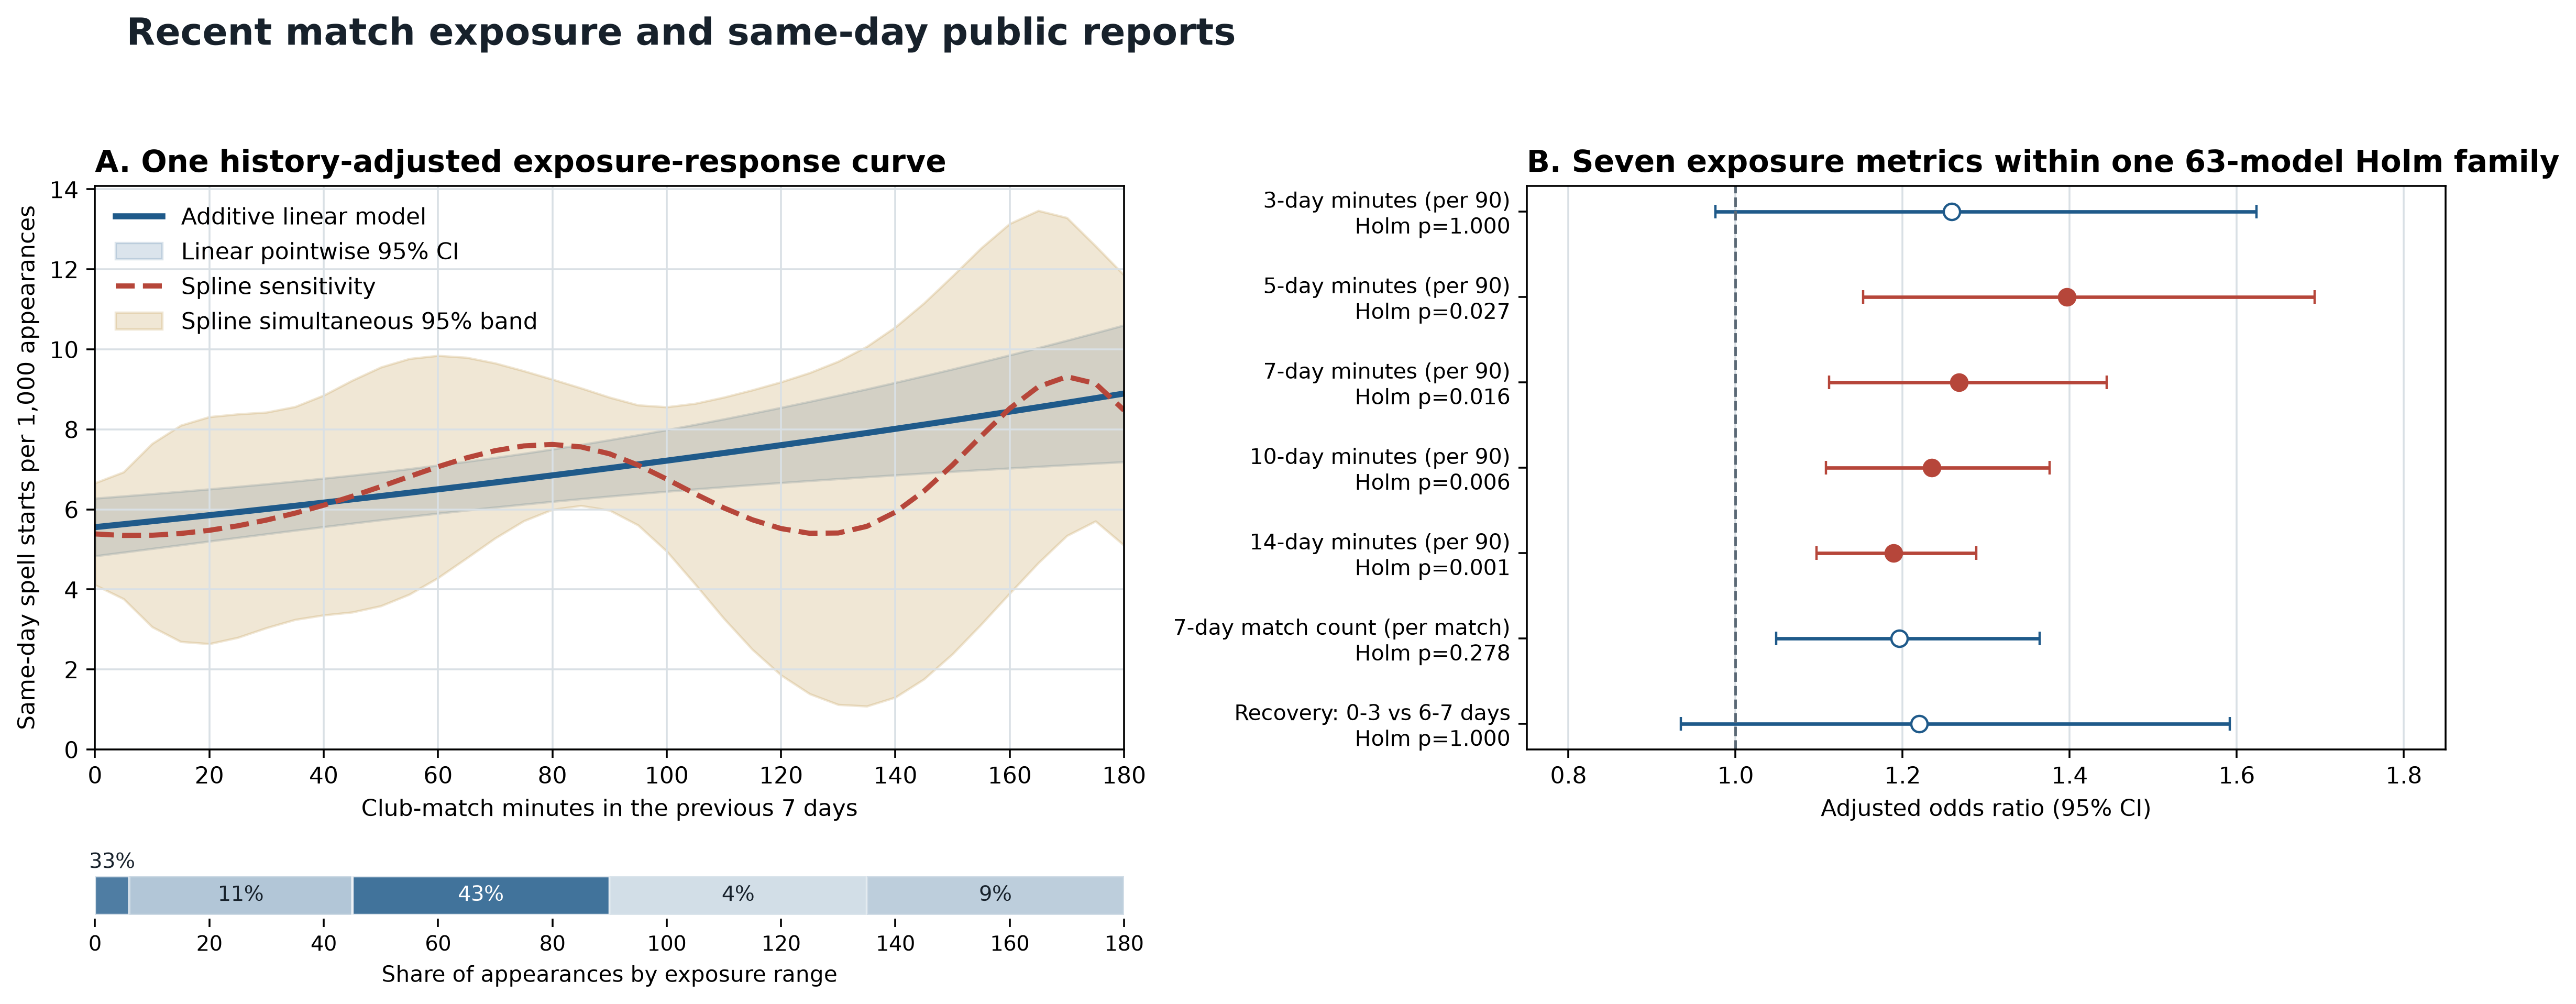
\includegraphics[width=\textwidth]{figures/J6_jsams_primary_robustness.png}
\caption{The worked-example exposure association and its alternative metrics, retained here because the association is the thing being divided rather than a finding of this paper. Panel A shows one additive history-adjusted curve, standardised over observed calendar phases with prior history fixed at its sample median; the linear model has pointwise 95\% confidence intervals and the flexible spline sensitivity a simultaneous 95\% band over 0--180 minutes. The band beneath panel A gives the share of appearances in each exposure range, so the sparsely supported 91--180-minute region is visible; a third of appearances sit at exactly zero recent minutes. Panel B gives player-clustered odds ratios for seven same-day per-appearance exposure metrics. The five cumulative windows overlap by construction and are correlated sensitivity analyses around the seven-day reference, not independent replications; filled points fell below one Holm threshold spanning all 63 exposure, timing and denominator models.}
\label{fig:supp_primary}
\end{figure}

\section{Measured confounding and clustering}

The reference model adjusts prior report history and calendar phase only. Table~\ref{tab:supp_confounding} refits it with measured covariates added singly and together, restricted to Premier League matches, and under two alternative clustering schemes. No variant in Table~\ref{tab:supp_confounding} moved the estimate outside 1.27--1.32 and none crossed one; the club-schedule refits shown alongside them in Fig.~\ref{fig:supp_robustness}A sit higher, at 1.36--1.39, because schedule and individual minutes are collinear by construction, and the temporal blocks in panel B carry wider intervals that cross one --- both are discussed in their own sections below. This bounds measured confounding; it says nothing about unmeasured health, symptoms or medical decisions.

\begin{figure}[h]
\centering
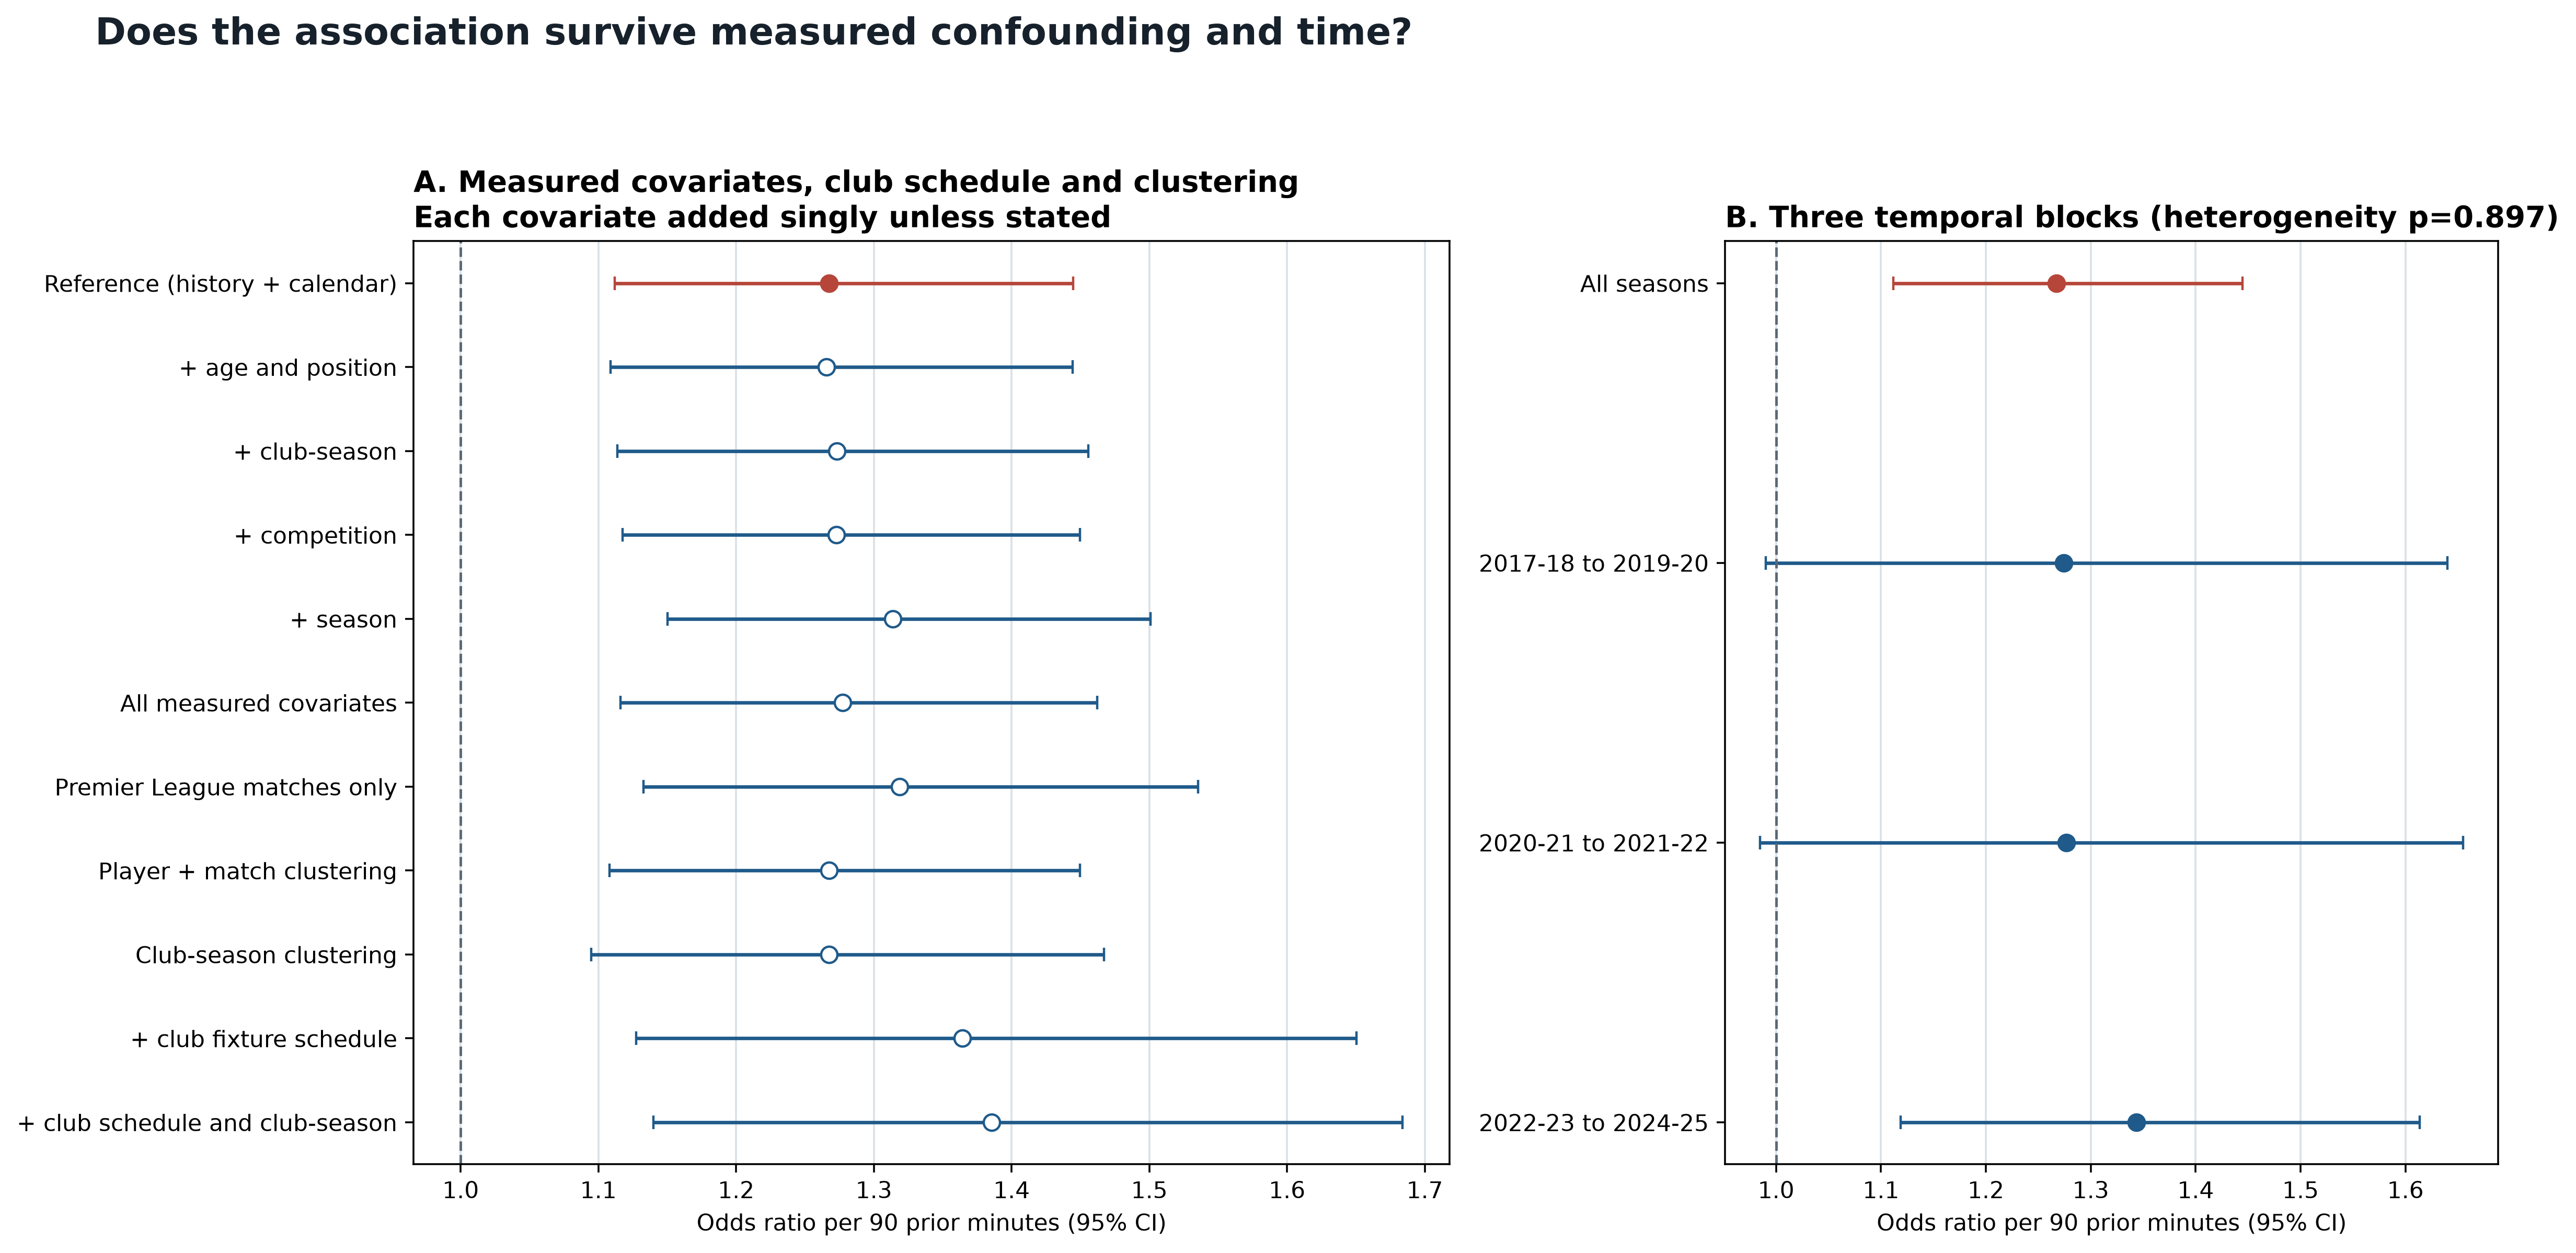
\includegraphics[width=\textwidth]{figures/J3_jsams_within_player_lineup_coverage.png}
\caption{Robustness of the reference estimate. Panel A refits the reference model with measured covariates added singly and together, restricted to Premier League matches, with club fixture gap and club fixture count, with club-season fixed effects, and under player-and-match and club-season clustering; the red point is the reference model. Panel B gives the overall and three fixed-block odds ratios per 90 previous-seven-day minutes, with a heterogeneity test asking whether slopes differ across blocks.}
\label{fig:supp_robustness}
\end{figure}

\begin{table}[h]
\centering
\caption{Measured-confounding and clustering sensitivity for the reference seven-day estimate. Odds ratios are per 90 previous-seven-day minutes with 95\% confidence intervals.}
\label{tab:supp_confounding}
\small
\begin{tabular}{llc}
\toprule
Specification & Uncertainty & Odds ratio (95\% CI)\\
\midrule
Reference (history + calendar) & Player & 1.27 (1.11--1.44)\\
\quad + age and position group & Player & 1.27 (1.11--1.44)\\
\quad + club-season & Player & 1.27 (1.11--1.46)\\
\quad + current-match competition & Player & 1.27 (1.12--1.45)\\
\quad + season & Player & 1.31 (1.15--1.50)\\
All measured covariates & Player & 1.28 (1.12--1.46)\\
Premier League matches only & Player & 1.32 (1.13--1.54)\\
Reference model & Player + match & 1.27 (1.11--1.45)\\
Reference model & Club-season & 1.27 (1.09--1.47)\\
\bottomrule
\end{tabular}
\end{table}

\section{Absolute risk and exposure support}

Standardised probabilities describe appearances by established players, averaged over the observed calendar-phase distribution with continuous prior history fixed at its sample median. The fitted probability was 5.56 per 1,000 appearances (95\% CI 4.84--6.28) at zero previous-seven-day minutes and 8.89 (7.19--10.60) at 180, a difference of 3.34 per 1,000 (1.31--5.37) by the delta method.

Support is uneven. Zero minutes covers 29,344 appearances (33.1\%, 162 same-day starts), 1--45 minutes 9,841 (11.1\%, 58), 46--90 minutes 37,905 (42.8\%, 273), 91--135 minutes 3,593 (4.1\%, 20) and 136--180 minutes 7,709 (8.7\%, 63). Above 180 minutes there were 181 appearances (0.2\%) and no same-day starts, so that region is excluded from every displayed curve.

\section{Selection: leakage gates and population}

Every covariate in the appearance-selection model is fixed before the fixture, and no outcome column enters it. A spell start recorded on an appearance date never removes that appearance, because public episodes mark unavailability only from the day after onset. Automated gates confirmed that all 65,100 Premier League appearances and all 401 of their same-day spell starts were retained in the opportunity set. The 12,348 appearances outside the set are in other competitions, which have no reconstructed EPL fixture; this restricts scope rather than conditioning on the outcome.

The included set contained 65,100 appearances by 1,112 players with 401 same-day starts (6.2 per 1,000); the excluded set contained 23,473 appearances by 1,086 players with 175 starts (7.5 per 1,000). Median previous-seven-day minutes were 75 versus 74 and median age 27.0 versus 26.7 years.

\section{Temporal refits}

The additive seven-day model was locked before splitting the study window. The early block retained 26,928 appearances, 633 players and 150 same-day reports; its odds ratio per 90 minutes was 1.27 (95\% CI 0.99--1.64; Holm $\pval=0.119$). The middle block retained 25,227 appearances, 648 players and 118 reports; its ratio was 1.28 (0.98--1.65; $\pval=0.119$). The late block retained 36,418 appearances, 755 players and 308 reports; its ratio was 1.34 (1.12--1.61; $\pval=0.005$). The global slope-by-block interaction was $\pval=0.897$. Blocks had separate rows but could share players, so they are internal temporal checks rather than independent prospective cohorts.

\section{Independent-source outcome audit}

The deterministic sample contained ten non-severe muscle/tendon reports, ten other non-severe reports and ten reports with at least 28 reported absence days. The hash-based selection file, as issued to the searcher, contained player, date, club and report text but no exposure value or fitted result. One author searched club, league and contemporaneous news sources independent of Transfermarkt. Automated gates confirmed exact queue keys and immutable fields, no exposure fields, an independent source for every resolved row and no Transfermarkt source. The selection had to be made on real identifiers, because the sample is drawn by hashing them; identity is removed afterwards, so the deposited copy of that file carries a surrogate record key, a surrogate player key and the season in place of the player, the club and the date, and records whether a qualifying source was found rather than its address. Thus source independence does not mean independent clinical adjudication or a second assessor.

Date attribution was \emph{confirmed} only when an independent source linked a new condition to the sampled appearance. A documented pre-existing condition or contradictory timing was \emph{not confirmed}; no adequate source was \emph{unresolved}. Description consistency used the same three verdicts but compared the public label with the independent description. This protocol estimates agreement among sampled reported positives. It cannot measure unreported cases, clinical diagnosis or inter-rater agreement.

\begin{table}[h]
\centering
\caption{Independent public-source audit. Confirmed proportions use resolved records as the denominator and Wilson 95\% confidence intervals. Unresolved counts remain visible.}
\label{tab:supp_audit}
\small
\begin{tabular}{llccc}
\toprule
Dimension & Stratum & Confirmed/resolved & Proportion (95\% CI) & Unresolved\\
\midrule
Date & Muscle/tendon, $<28$ days & 8/9 & 88.9\% (56.5--98.0) & 1\\
Date & Other, $<28$ days & 7/9 & 77.8\% (45.3--93.7) & 1\\
Date & Reported absence $\geq28$ days & 9/9 & 100\% (70.1--100) & 1\\
Date & All strata & 24/27 & 88.9\% (71.9--96.1) & 3\\
Description & Muscle/tendon, $<28$ days & 8/9 & 88.9\% (56.5--98.0) & 1\\
Description & Other, $<28$ days & 5/8 & 62.5\% (30.6--86.3) & 2\\
Description & Reported absence $\geq28$ days & 10/10 & 100\% (72.2--100) & 0\\
Description & All strata & 23/27 & 85.2\% (67.5--94.1) & 3\\
\bottomrule
\end{tabular}
\end{table}

\begin{table}[h]
\centering
\caption{The same audit expressed over every sampled record. Because unresolved records could fall either way, the bounds assume they are all not confirmed (low) or all confirmed (high).}
\label{tab:supp_audit_sampled}
\small
\begin{tabular}{lcccc}
\toprule
Dimension & Confirmed/sampled & Proportion (95\% CI) & Lower bound & Upper bound\\
\midrule
Date attribution & 24/30 & 80.0\% (62.7--90.5) & 80.0\% & 90.0\%\\
Description consistency & 23/30 & 76.7\% (59.1--88.2) & 76.7\% & 86.7\%\\
\bottomrule
\end{tabular}
\end{table}


\begin{figure}[p]
\centering
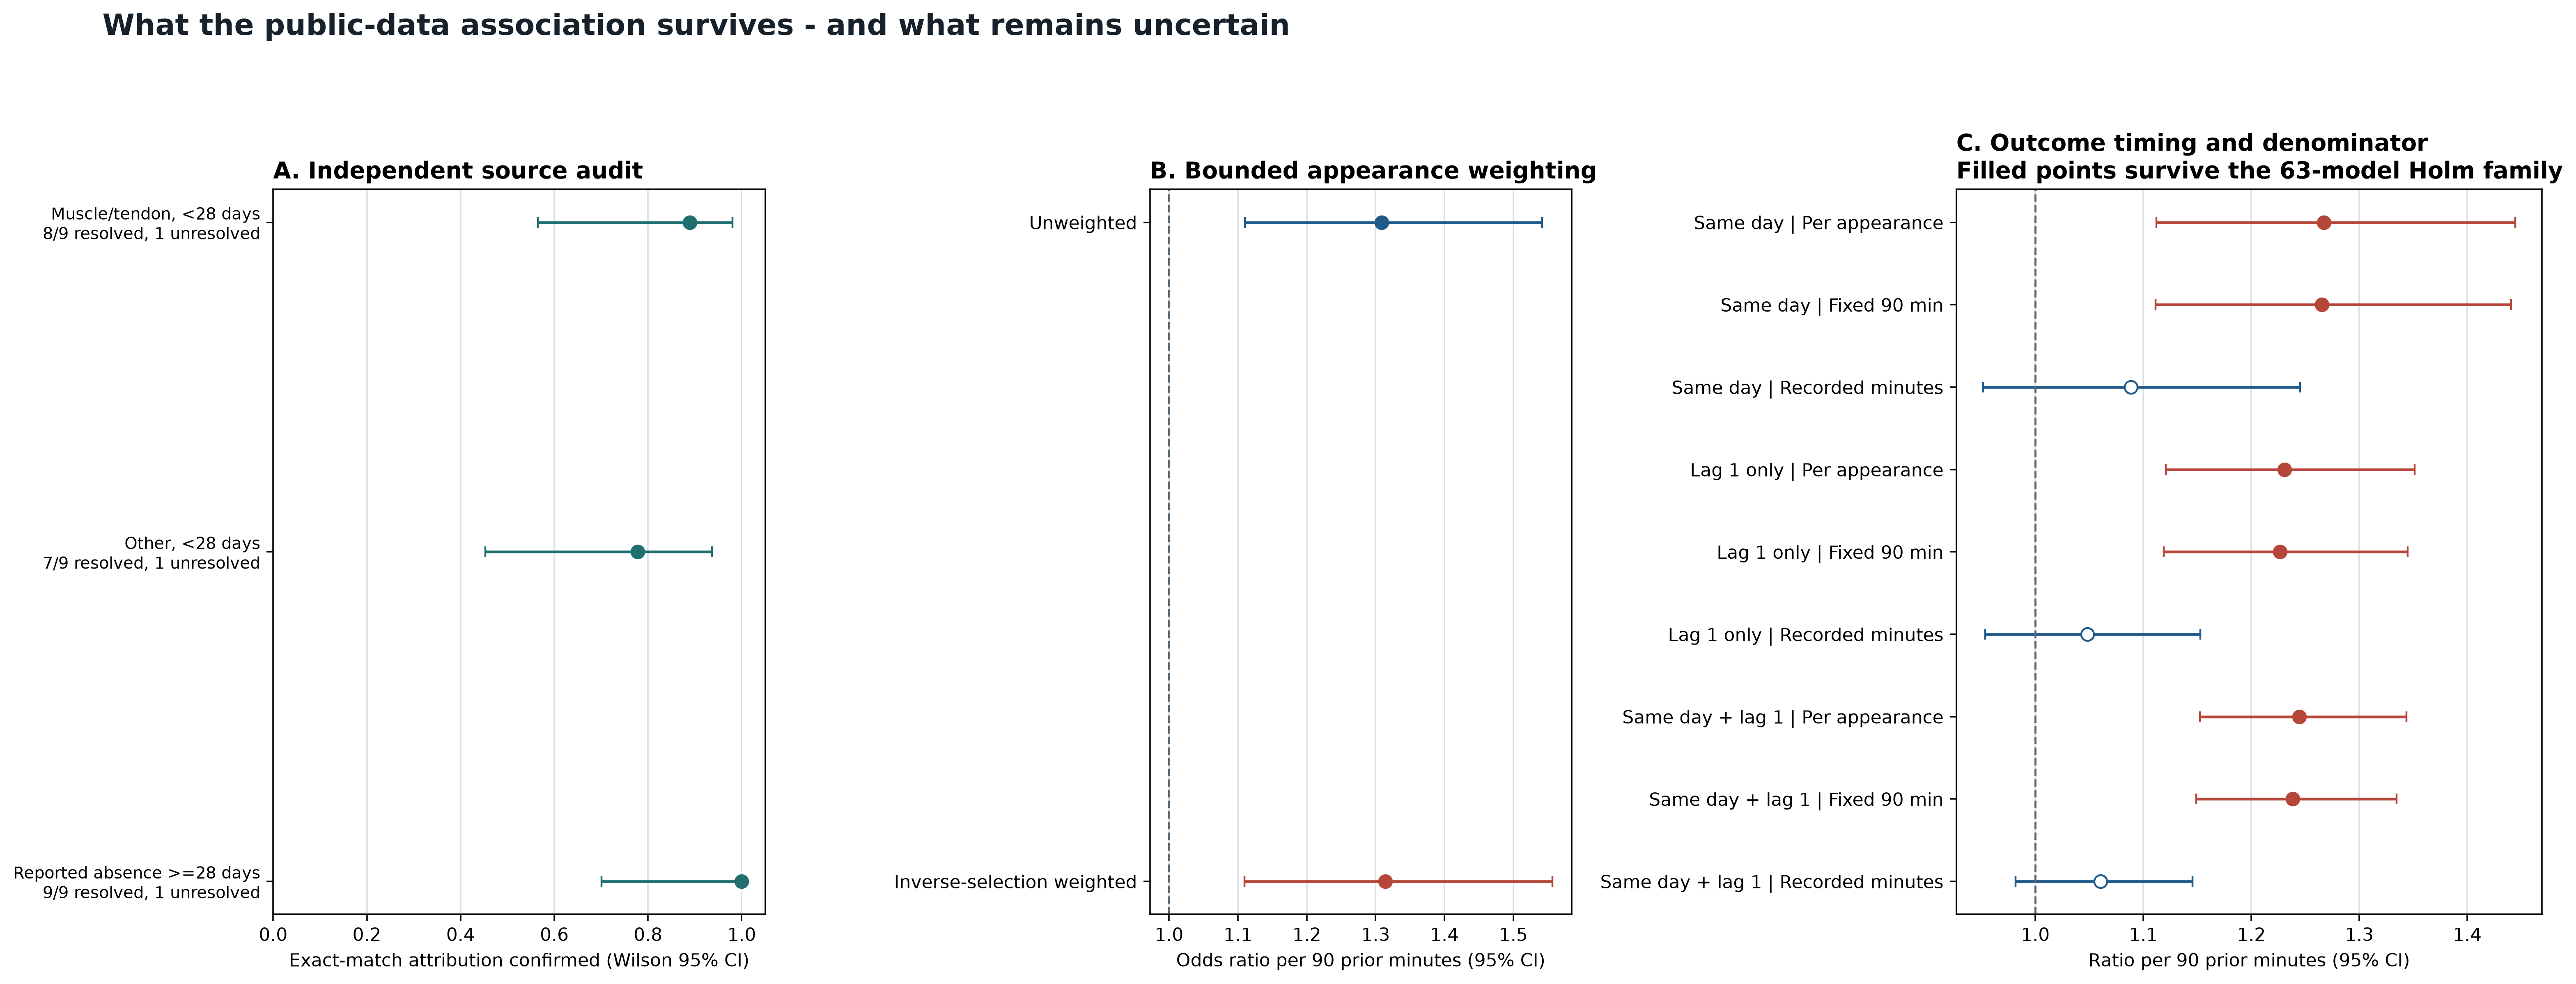
\includegraphics[width=\textwidth]{figures/J4_jsams_context_support.png}
\caption{Outcome attribution and structural sensitivities. Panel A gives Wilson 95\% intervals for exact-match attribution among independently resolved sampled records; each stratum also had one unresolved record, and the all-sampled proportion is bounded between 80.0\% and 90.0\%. Panel B compares the seven-day association before and after restricted measured-selection weighting inside the bounded Premier League opportunity set. Panel C compares outcome timing and denominator for the seven-day metric; filled points fell below the common 63-model Holm threshold. Per-appearance odds ratios and minute-based incidence-rate ratios answer different questions.}
\label{fig:supp_audit}
\end{figure}

\section{Missed events and inter-rater agreement: searched, unresolved}

The audit above samples only reported positives, so it cannot estimate the events the public record missed. We therefore generated a second deterministic, exposure-blinded queue of 30 appearances carrying \emph{no} same-day spell start, drawn by hashed player-date identifier from the same eligible cohort and containing player, date, club and match context but no exposure value or fitted result. As above, the deposited copy replaces the first three with surrogate keys and a season.

That queue has now been searched under the pre-specified protocol deposited as \path{jsams_revised_missed_event_adjudication_protocol.csv}, whose rules B1--B7 fix the admissible sources, the temporal window, the specificity required, the identification standard, the verdict set, the assessors, and --- decisively --- that failure to find a source maps to \emph{unresolved} and never to \emph{no missed event}.

Searching first required knowing which records could be searched at all, and the screen that answers this is the more useful result. Counting days elapsed is uninformative, because in this calendar every long gap coincides with a scheduled break. Counting \emph{club fixtures missed} is not. \path{jsams_revised_non_event_absence_screen.csv} asks, for each queued appearance, how many fixtures the player's club played before that player next appeared. In 28 of the 30 the club played none: there was no absence for a report to have missed, so the record cannot be evidence of under-ascertainment. Of the remaining two, one gap spans a club change, so the missed fixtures are not absences; for the other the only public source is dated nine days after the appearance and describes an assessment rather than an injury, which rule B2 excludes. The screen assigns no verdicts and cannot: a player can be injured and miss nothing.

The outcome is therefore 30 sampled, 30 unresolved, 0 resolved, and \path{jsams_revised_non_event_audit_summary.csv} records its status as \emph{reviewed, not resolved} rather than complete. The deposited queue file \path{jsams_revised_non_event_audit_queue.csv} preserves the blinded artifact exactly as issued to the searcher, its verdict column still reading \emph{pending}; the verdicts themselves live in the manual review file under \path{data/manual/}, and the summary reads them from there, so the two files describe the same records at different moments rather than disagreeing. Both are keyed by the same surrogates, which is what still joins a verdict to the appearance it judges once the identifiers are gone. The missed-event proportion and its Wilson interval remain \emph{unestimated} and the outcome's sensitivity is unknown. Zero confirmed missed events is not an estimate of zero. The same applies to reliability: \path{jsams_revised_second_assessor_agreement.csv} records zero compared rows, because no second assessor's codes exist, so Cohen's kappa for date attribution is unestimated. Both quantities are computed automatically by the archived code as soon as verdicts are supplied; we report them as unestimated rather than substituting a weaker proxy.

\section{Recorded-minute denominator}

Same-day rows averaged 50.06 minutes and non-event appearances 71.10; their difference was $-21.05$ minutes (95\% player-bootstrap interval $-23.10$ to $-19.02$). In the six seasons with complete lineup data, starters differed by $-31.19$ ($-33.88$ to $-28.62$) minutes and substitutes by 2.15 ($-3.01$ to 7.48). Standardising both groups over the pooled lineup mix gave $-24.66$ ($-27.05$ to $-22.20$). These comparisons show outcome-linked exposure recording; they do not reveal event minute or time lost.

\begin{table}[h]
\centering
\caption{Recorded minutes by lineup role and event status. Truncation should appear as a shifted distribution among starters and as no shift among substitutes, whose recorded minutes are set by when they came on rather than when they left.}
\label{tab:supp_minute_distribution}
\small
\begin{tabular}{llrrrrrr}
\toprule
Role & Event status & $n$ & p10 & p25 & Median & p75 & p90\\
\midrule
Starters & No same-day report & 53,626 & 68 & 89 & 90 & 90 & 90\\
Starters & Same-day spell start & 364 & 21 & 36 & 53 & 74 & 90\\
Substitutes & No same-day report & 13,304 & 3 & 9 & 18.0 & 27 & 45\\
Substitutes & Same-day spell start & 26 & 5.5 & 11 & 18.5 & 30 & 43\\
Lineup unknown & No same-day report & 21,067 & 14 & 45 & 90 & 90 & 90\\
Lineup unknown & Same-day spell start & 186 & 15 & 26 & 45 & 66 & 87\\
\bottomrule
\end{tabular}
\end{table}

The difference does not depend on which seasons carry lineup data. It was $-20.42$ minutes inside the complete-lineup era (2017--18 to 2022--23; 64,387 appearances, 360 events) and $-20.86$ outside it (24,186 appearances, 216 events), and $-20.32$ where lineup status is known against $-21.40$ where it is not. The starter and substitute split is therefore not an artefact of lineup coverage.

\section{Why a minute denominator attenuates the exposure association}

For a Poisson model with a log-minutes offset, $\log E[y]=\log(m)+a+b_{\text{off}}x$, while the same model without the offset gives $\log E[y]=a'+b_{\text{app}}x$. To first order $b_{\text{off}}=b_{\text{app}}-\gamma$, where $\gamma$ is the slope of $\log(m)$ on the exposure. The attenuation caused by dividing by minutes is therefore predicted by $\gamma$ alone, and $\gamma$ has two possible sources: outcome truncation, and ordinary dependence of appearance length on the exposure.

\begin{table}[h]
\centering
\caption{Decomposition of the minute-denominator attenuation. Values are on the log scale unless stated. The counterfactual replaces each event row's minutes with the mean for non-event appearances of the same lineup role, removing truncation and leaving exposure-dependence intact.}
\label{tab:supp_attenuation}
\small
\begin{tabular}{lr}
\toprule
Quantity & Value\\
\midrule
$\gamma$, slope of log recorded minutes on exposure & 0.3032\\
$\gamma$ with truncation removed & 0.3036\\
$\gamma$ attributable to outcome truncation & $-0.0004$\\
Truncation share of $\gamma$ & $-0.13\%$\\
$\gamma$ within starters only & 0.0106\\
$\gamma$ within substitutes only & 0.2140\\
Observed attenuation, fixed-90 minus recorded minutes & 0.1506\\
Minutes lost to truncation & 15,259\\
Truncation share of all recorded minutes & 0.243\%\\
Rate inflation factor from truncation & 1.0024\\
\bottomrule
\end{tabular}
\end{table}

Outcome truncation explains essentially none of the attenuation: it accounts for $-0.13\%$ of $\gamma$, and the minutes it removes are 0.243\% of the total, because same-day reports occur on only 0.65\% of appearances.

\subsection*{The identity over-predicts, and the direct refit does not}

The identity is a first-order expansion, and in these data it over-predicts. It implies an attenuation equal to $\gamma=0.3032$; the attenuation actually observed between the fixed-90 and recorded-minute models is 0.1506, so the identity over-states it by a factor of 2.01. The discrepancy tracks the size of $\gamma$: within starters it predicts 0.0106 against 0.0120 observed, essentially exact, while within substitutes it predicts 0.2140 against 0.1165, off by 1.8. The expansion weights every appearance equally, whereas the Poisson score weights by fitted means, so the attenuation follows the minutes--exposure gradient among event-bearing rows rather than across the whole panel. The identity is therefore trustworthy for the \emph{ratio} it is used for here and untrustworthy for the magnitude.

We therefore measure the truncation contribution without any expansion. The same Poisson model is fitted twice, changing nothing but the offset: recorded minutes, then the same minutes with truncation removed. Rows, family, link, covariates and clustering are identical.

\begin{table}[h]
\centering
\caption{Direct truncation refit. One model, three offsets, everything else held fixed. The gap between the recorded-minute and untruncated-minute fits is the truncation contribution itself, not a prediction of it.}
\label{tab:supp_direct_refit}
\small
\begin{tabular}{lccr}
\toprule
Offset & Estimate (95\% CI) & Log estimate & \\
\midrule
Recorded minutes & 1.0884 (0.9515--1.2450) & 0.08472 & \\
Untruncated minutes & 1.0883 (0.9516--1.2445) & 0.08457 & \\
Fixed 90 minutes & 1.2653 (1.1112--1.4408) & 0.23533 & \\
\midrule
\multicolumn{3}{l}{Gap, untruncated minus recorded} & $-0.00014$\\
\multicolumn{3}{l}{Total attenuation, fixed-90 minus recorded} & $0.15061$\\
\multicolumn{3}{l}{Truncation share of the attenuation} & $-0.095\%$\\
\bottomrule
\end{tabular}
\end{table}

The direct estimate ($-0.095\%$) and the analytic one ($-0.13\%$) agree, so the attribution does not depend on the identity. Readers applying this arithmetic to their own data should use the direct comparison.

\subsection*{Where truncation does matter}

A whole-cohort denominator dilutes a rare-event distortion in proportion to how rare the events are. Restricting to the appearances that carry an event removes that protection entirely.

\begin{table}[h]
\centering
\caption{The same truncation, two populations. Recorded exposure is understated by a factor of roughly 143 more on case-restricted quantities than on the cohort as a whole.}
\label{tab:supp_case_restricted}
\small
\begin{tabular}{lrrr}
\toprule
Quantity & Observed & Truncation removed & Understated by\\
\midrule
Mean recorded minutes, event appearances & 50.06 & 76.55 & 34.61\%\\
Total recorded minutes, whole cohort & 6,285,729 & 6,300,988 & 0.24\%\\
\bottomrule
\end{tabular}
\end{table}

Any quantity conditioned on cases --- exposure on the day of injury, minutes before an event, or a burden or severity measure denominated on the injured players' own recorded time --- carries the 34.6\% distortion rather than the 0.24\% one.

\subsection*{How much of that is the imputation?}

The counterfactual minutes are a modelling choice, and the case-restricted figure is a mean against an imputed mean, so the choice is the answer rather than a detail of it. Table~\ref{tab:supp_imputation} repeats every truncation quantity under five schemes.

\begin{table}[h]
\centering
\caption{Truncation quantities under alternative imputations of the untruncated minutes. The case-restricted distortion moves across schemes; the attribution does not.}
\label{tab:supp_imputation}
\small
\begin{tabular}{lrrr}
\toprule
Imputation of event-row minutes & Case-restricted & Cohort & Truncation share\\
 & understated & understated & of attenuation\\
\midrule
Role mean (reference) & 34.61\% & 0.242\% & $-0.09\%$\\
Role median & 42.30\% & 0.335\% & $-0.10\%$\\
Role 75th percentile & 42.57\% & 0.339\% & $-0.08\%$\\
Role and exposure band, mean & 34.76\% & 0.244\% & $-0.36\%$\\
Role and season, mean & 34.55\% & 0.242\% & $-0.09\%$\\
\bottomrule
\end{tabular}
\end{table}

Two things follow. The case-restricted distortion ranges from 34.5\% to 42.6\%, and the headline 34.6\% sits at the least-alarming end of that range rather than the most: matching on role and season shaves it marginally, to 34.55\%, while the role median and the role 75th percentile make it larger. The cohort figure moves correspondingly little, from 0.242\% to 0.339\%. And the attribution is stable under every scheme, with truncation explaining between $-0.08\%$ and $-0.36\%$ of the attenuation, so no imputation choice available to us disturbs the conclusion that truncation is not what attenuates the exposure association.

What the schemes cannot address is that event appearances may differ from non-event appearances for reasons unrelated to the event --- a player withdrawn for performance, a decided match, a rotation game. Matching on role, exposure band or season narrows that gap without closing it, and the case-restricted figure should be read as an order of magnitude rather than a point estimate. What does explain it is composition. Within starters, $\gamma$ is 0.0106 and within substitutes 0.2140, yet pooled it is 0.3032, because the share of appearances that are starts is higher at high exposure than at low (Table~\ref{tab:supp_composition}). Recorded minutes are therefore a consequence of the exposure, and dividing by them removes part of the gradient under study.

\begin{table}[h]
\centering
\caption{Squad role and appearance length by exposure band. Both the share of starts and mean recorded minutes are substantially higher in the high-exposure bands than in the low, which is why recorded minutes are a function of the exposure. Neither series is monotonic across bands: both dip at 1--45 minutes, where a player who played briefly last week is likely to be a substitute again, and again at 91--135, a band holding only 4\% of appearances. $\gamma$ summarises this as an average linear gradient and should not be read as a step-by-step rise.}
\label{tab:supp_composition}
\small
\begin{tabular}{lrrr}
\toprule
Previous-7-day minutes & Appearances & Share starting & Mean recorded minutes\\
\midrule
0 & 29,344 & 55.5\% & 66.4\\
1--45 & 9,841 & 40.9\% & 54.0\\
46--90 & 37,905 & 69.2\% & 77.4\\
91--135 & 3,593 & 55.8\% & 69.6\\
136--180 & 7,709 & 69.1\% & 78.5\\
$>$180 & 181 & 70.2\% & 83.2\\
\bottomrule
\end{tabular}
\end{table}




\subsection*{Adjusting for squad role is not stratifying by it}

The main text recommends analysing within starters. A natural question is whether adjusting for squad role would do instead, since adjustment keeps the whole cohort. It would not, and the reason is structural rather than empirical: a categorical role term enters the linear predictor, while the offset $\log(m)$ keeps every bit of its within-role variation. Restricting to starters works because it selects rows whose offset barely moves ($\gamma=0.011$, interquartile range two minutes); adjusting selects nothing.

\begin{table}[h]
\centering
\caption{The denominator comparison with squad role adjusted rather than stratified, on all 88,573 appearances and 576 events. Both models are Poisson with a log link on identical rows; the adjusted pair adds one categorical role term to each. Adjustment removes about half the attenuation and leaves six times what restricting to starters leaves. Attenuation intervals are percentile intervals from resampling players 1,000 times, the same procedure used for the strata.}
\label{tab:supp_role_adjusted}
\small
\begin{tabular}{llrl}
\toprule
Model & Denominator & Estimate (95\% CI) & Attenuation\\
\midrule
Unadjusted & Fixed 90 minutes & 1.265 (1.111--1.441) & \multirow{2}{*}{0.151 (0.140--0.163)}\\
Unadjusted & Recorded minutes & 1.088 (0.951--1.245) & \\
Adjusted for squad role & Fixed 90 minutes & 1.185 (1.037--1.354) & \multirow{2}{*}{0.071 (0.062--0.080)}\\
Adjusted for squad role & Recorded minutes & 1.104 (0.965--1.262) & \\
\bottomrule
\end{tabular}
\end{table}

Adjustment is not useless: 0.151 falls to 0.071, so a role term absorbs the part of the offset gradient that runs between roles. It leaves the part that runs within them, which is most of what remains. The three attenuations are cleanly separated --- 0.140 to 0.163 pooled, 0.062 to 0.080 adjusted, 0.009 to 0.015 within starters --- so the ordering is not an artefact of reading point estimates against each other. A reader who cannot stratify should therefore report per-appearance risk rather than assume a covariate has repaired the denominator.

This also explains why the two operations coincide in a panel where minutes are constant inside each role and diverge in a real one. What a role term can absorb is exactly the between-role component; everything the interquartile ranges in Table~2 of the main text describe --- 18 minutes among substitutes, 45 where lineup status is unknown --- is left untouched.

\subsection*{Who the run-in removes}

Requiring 900 earlier club-match minutes is an eligibility choice, and it drops 350 of 1,558 source players. They are not a random fifth.

\begin{table}[h]
\centering
\caption{Players removed by the 900-minute run-in against those retained. Medians are over players; prior minutes are each player's maximum accumulated total.}
\label{tab:supp_run_in}
\small
\setlength{\tabcolsep}{4pt}
\begin{tabular}{lrrrrr}
\toprule
 & & & \multicolumn{3}{c}{Median per player}\\
\cmidrule(l){4-6}
Population & Players & Appearances & Age & Appearances & Prior minutes\\
\midrule
Excluded by the run-in & 350 & 2,586 & 22.6 & 5.0 & 180\\
Retained at the run-in & 1,208 & 98,456 & 26.7 & 56.5 & 6,598\\
\bottomrule
\end{tabular}
\end{table}

The excluded are young players with a handful of senior appearances between them: 2,586 appearances across 350 players, against 98,456 across 1,208. The cohort's 88,573 eligible rows are fewer than the retained players' 98,456 because a retained player's own appearances before he crosses 900 minutes are excluded too: those 9,883 rows, plus the 2,586 from excluded players, are the 12,469 the main text removes. The restriction buys a cohort with enough prior exposure for a history term to mean anything, at the cost of saying nothing about players in their first season of senior football. The association at 450 and 1,800 minutes is reported below and is similar at both.

\subsection*{Uncertainty on $\gamma$}

$\gamma$ carries the composition argument in the substitute stratum, where 26 events leave the association itself uninformative, so it needs an interval of its own. Every $\gamma$ below is an ordinary least-squares slope of log recorded minutes on exposure over the same covariates as the reference model, fitted with player-clustered standard errors. The pooled and within-stratum fits use the same estimator, so the four values may be compared with each other.

\begin{table}[h]
\centering
\caption{Player-clustered 95\% intervals for the exposure-dependence of appearance length. $\gamma$ is estimated from rows rather than events, which is why the substitute and unknown-lineup strata are precisely estimated here despite carrying 26 and 186 events. The within-starter interval is disjoint from all three others.}
\label{tab:supp_gamma}
\small
\begin{tabular}{lrrl}
\toprule
Stratum & Appearances & $\gamma$ & 95\% interval\\
\midrule
All appearances & 88,573 & 0.3032 & 0.2834 to 0.3230\\
Starters & 53,990 & 0.0106 & 0.0074 to 0.0138\\
Substitutes & 13,330 & 0.2140 & 0.1815 to 0.2466\\
Lineup unknown & 21,253 & 0.3513 & 0.3170 to 0.3856\\
\bottomrule
\end{tabular}
\end{table}

The separation is complete where the argument needs it. The within-starter interval reaches 0.0138, and the next-lowest stratum starts at 0.1815, so the gap between starters and every other stratum is more than a factor of ten and no interval comes near closing it. Pooled and unknown-lineup overlap marginally (0.3230 against 0.3170), which is expected: rows with no lineup status are a quarter of the panel and carry the largest $\gamma$ in it, so they pull the pooled value towards themselves.

This is the cleanest form of the composition claim, because it involves the outcome nowhere. $\gamma$ describes only how appearance length varies with exposure. That it is near zero among starters and large everywhere else establishes the mechanism without any model of injury at all; the attenuation results then show that the mechanism has the consequence we say it has.

\subsection*{Is $\gamma$ an artefact of the log, the floor or the ceiling?}

The reference fit takes least squares on the log of recorded minutes, clipped below at one minute. Neither the transform nor the floor is beyond question. Minutes are bounded above at a full appearance and heap on it --- among starters the interquartile range is two minutes --- so the response is close to a point mass, and a one-minute substitute appearance sits far out on a log scale. Both choices were therefore varied, on Premier League appearances under the cross-league diagnostic specification.

Raising the floor from one minute to five and then ten moved the pooled gradient from 0.472 to 0.421 to 0.377 while the within-starter gradient held at 0.020 throughout. The floor moves the level and leaves the contrast untouched, which is what the claim depends on.

Three alternative estimators were then fitted: quantile regression at the median, which ignores the heap; a binomial fit on minutes as a share of a full appearance, which respects the ceiling; and least squares among appearances short of the ceiling. Their pooled gradients were 0.022, 1.212 and 0.633 against the reference 0.472, and their within-starter gradients 0.000, 0.294 and $-0.010$ against 0.020. Two things follow, and the second is a caution.

The level of $\gamma$ is strongly specification-dependent and should not be quoted as though it were not. The median fit is the extreme case and is the most instructive: the median appearance is a full one at almost every exposure, so the median barely moves and its gradient nearly vanishes. That is not a contradiction. The attenuation identity runs on the \emph{mean} of log minutes, not the median, so least squares is the estimand the arithmetic requires, and the median fit instead bounds how much of the gradient is carried by the typical appearance rather than by the changing mix of appearance types. The answer is almost none of it: the gradient is a composition effect, exactly as the paper argues.

The contrast, which is what the paper claims, survives every estimator in which it can be interpreted. The ceiling-excluding fit is excluded from that statement rather than counted towards it, and the reason matters: dropping the ceiling from the starter stratum retains precisely the appearances that ended early, which is the truncation measured elsewhere in this supplement. It yields a number and the number answers a different question, so \path{jsams_revised_denominator_gradient_estimator_sensitivity.csv} flags it as not interpretable rather than allowing it to support a claim it cannot address.

\subsection*{Correlations among the cumulative windows}

The five cumulative windows share matches by construction. Across the ten pairs the Pearson correlation runs from 0.361 (three against fourteen days) to 0.846 (ten against fourteen), and the manuscript quotes that full range. An earlier draft quoted 0.68 to 0.83, which was the range over the subset of pairs involving the seven-day reference and excluding the three-day window, and did not match the ``up to 0.85'' quoted in the Discussion. Both now refer to the same ten pairs, and \path{exposure_metric_correlations.csv} flags them with \path{both_cumulative_windows} so the range is auditable.

The spread is itself informative. The three-day window is the least correlated with the others and is also the one window whose association does not clear the Holm threshold, which is consistent with the precision reading below rather than with a shorter window carrying a different signal.

\subsection*{Does squad role generate the association as well as the offset?}

Recorded minutes track exposure through squad role, so the association itself may partly reflect who is selected rather than what playing does. The reference per-appearance model was therefore refitted unadjusted, adjusted for lineup role on identical rows, and within each role.

\begin{table}[h]
\centering
\caption{The reference seven-day association under squad-role adjustment and stratification. Adjusting adds one categorical term to the same 88,573 rows, so the movement between the first two rows is role composition. The within-starter estimate is reported to three decimal places because rounding its lower bound to 1.00 would disguise an interval that crosses the null.}
\label{tab:supp_role_association}
\small
\begin{tabular}{lrrr}
\toprule
Analysis & Odds ratio (95\% CI) & $\pval$ & Events\\
\midrule
Pooled, unadjusted for squad role & 1.267 (1.112--1.445) & 0.0004 & 576\\
Pooled, adjusted for squad role & 1.186 (1.037--1.357) & 0.013 & 576\\
Within starters & 1.181 (0.998--1.398) & 0.052 & 364\\
Within substitutes & 1.301 (0.680--2.490) & 0.427 & 26\\
Where lineup status is unknown & 1.204 (0.945--1.535) & 0.133 & 186\\
\bottomrule
\end{tabular}
\end{table}

Squad role carries part of the association and not all of it. On the log scale the pooled coefficient falls from 0.237 to 0.171 on adjustment, so composition accounts for roughly 28\% of it; the main text reports the same movement as 1.27 to 1.19. What remains is marginal in the starter stratum, the one stratum in which the minute denominator can be trusted, and uninformative in the other two for want of events. We report this rather than setting it aside: it qualifies the worked example without touching the measurement claim, which concerns the offset and not the coefficient.

\subsection*{The gradient across cumulative windows is precision, not effect}

Adjusted $\pval$ values fall monotonically as the cumulative window lengthens, which invites the reading that longer windows carry a stronger signal --- and, since a player with high fourteen-day minutes is by construction an established starter, that the association is squad status in disguise. The point estimates do not support that reading.

\begin{table}[h]
\centering
\caption{The five cumulative exposure windows, per 90 minutes, on the same 88,573 appearances and 576 events. Holm values are from the single 63-model family. The odds ratio peaks at five days and declines thereafter while the standard error falls threefold, so what improves with window length is precision.}
\label{tab:supp_window_gradient}
\small
\begin{tabular}{lrrr}
\toprule
Window & Odds ratio (95\% CI) & Standard error & Holm $\pval$\\
\midrule
3 days & 1.259 (0.976--1.624) & 0.130 & 1.000\\
5 days & 1.397 (1.152--1.693) & 0.098 & 0.027\\
7 days & 1.267 (1.112--1.445) & 0.067 & 0.016\\
10 days & 1.235 (1.108--1.376) & 0.055 & 0.006\\
14 days & 1.189 (1.097--1.288) & 0.041 & 0.001\\
\bottomrule
\end{tabular}
\end{table}

Longer windows aggregate more matches, so the same per-90 exposure is measured with less noise: the standard error falls from 0.130 to 0.041 while the estimate drifts down from 1.40 to 1.19. The three-day window is not null because no signal is present there but because it cannot resolve one. A referee reading only the Holm column would infer a gradient in effect; there is none, and the two columns are printed together so that inference cannot be drawn.

\subsection*{Uncertainty on the attenuation}

The attenuation is a difference between two coefficients fitted to the same rows, and the composition argument compares that difference across strata, so neither quantity carries usable uncertainty from a single fit. Resampling players with replacement 1,000 times and refitting both offsets in every stratum gives percentile intervals.

\begin{table}[h]
\centering
\caption{Player-resampled percentile intervals for the denominator attenuation, in every stratum over which the remedy is claimed. Absolute attenuations are precisely estimated and cleanly separated; the same quantities expressed as a share of the estimate they act on are not, because each base estimate sits near or across the null. The stratum where lineup status is unknown carries the largest attenuation of all, and is the one in which stratifying by role is impossible.}
\label{tab:supp_attenuation_boot}
\small
\begin{tabular}{lrr}
\toprule
Quantity & Estimate & 95\% interval\\
\midrule
Pooled absolute attenuation & 0.1506 & 0.1400 to 0.1627\\
Within starters & 0.0120 & 0.0091 to 0.0147\\
Within substitutes & 0.1165 & 0.0775 to 0.1523\\
Where lineup status is unknown & 0.1805 & 0.1590 to 0.2018\\
\textbf{Pooled minus within-starter} & \textbf{0.1387} & \textbf{0.1285 to 0.1497}\\
\midrule
Pooled, as a share of the fixed-90 estimate & 0.640 & 0.418 to 1.355\\
Within starters, same scale & 0.072 & $-0.199$ to 0.446\\
Within substitutes, same scale & 0.444 & $-4.569$ to 4.234\\
Lineup unknown, same scale & 0.980 & $-6.334$ to 9.670\\
Ratio of pooled to within-starter share & 8.86 & $-0.67$ to 15.48\\
\bottomrule
\end{tabular}
\end{table}

The absolute comparison settles the question: pooled and within-starter attenuations do not overlap, and their difference is 0.139 (0.128--0.150), comfortably excluding zero. The relative comparison does not, and we report it to show why. Dividing by the fixed-90 estimate within starters divides by a quantity whose own interval touches the null, so the ratio inherits that instability and its interval spans one. An earlier draft claimed a ninefold relative difference that ``the modest gap in base estimates cannot produce''; the bootstrap shows that claim was not supported, and it has been replaced by the absolute difference, which is. Note also that within-starter is the only stratum in which the attenuation is removed. Substitutes retain 0.117 and rows with no lineup status retain 0.181, more than pooling costs, so the remedy is bounded to the stratum whose appearance length is nearly constant.

\begin{table}[h]
\centering
\caption{The three denominators refitted within squad role. Fixed-90 and recorded-minute models are both Poisson with a log link on identical rows, so only the offset differs. The pooled attenuation largely disappears within starters.}
\label{tab:supp_denominator_role}
\small
\begin{tabular}{llccr}
\toprule
Role & Denominator & Estimate (95\% CI) & Events & Log attenuation\\
\midrule
All & Per appearance & 1.267 (1.112--1.445) & 576 & \multirow{3}{*}{0.151}\\
All & Fixed 90 minutes & 1.265 (1.111--1.441) & 576 & \\
All & Recorded minutes & 1.088 (0.951--1.245) & 576 & \\
\midrule
Starters & Per appearance & 1.181 (0.998--1.398) & 364 & \multirow{3}{*}{0.012}\\
Starters & Fixed 90 minutes & 1.180 (0.998--1.395) & 364 & \\
Starters & Recorded minutes & 1.166 (0.987--1.378) & 364 & \\
\midrule
Substitutes & Per appearance & 1.301 (0.680--2.490) & 26 & \multirow{3}{*}{0.117}\\
Substitutes & Fixed 90 minutes & 1.300 (0.680--2.484) & 26 & \\
Substitutes & Recorded minutes & 1.157 (0.601--2.229) & 26 & \\
\bottomrule
\end{tabular}
\end{table}

\section{What the source records}

The pre-specified illness negative control could not be fitted because the eligible panel contained one same-day illness report. That scarcity is a property of the design rather than of the source: illness is recorded at a reasonable rate across all reconciled episodes, but it withdraws a player from the squad instead of ending a match he has started, so a same-day design cannot observe it.

\begin{table}[h]
\centering
\caption{Public label of every reconciled episode ($n=11{,}993$), classified by the same routine used for outcome-quality restrictions.}
\label{tab:supp_episode_types}
\small
\begin{tabular}{lrr}
\toprule
Episode label & Episodes & Share\\
\midrule
Muscle/tendon & 4,339 & 36.2\%\\
Other or unspecified & 3,028 & 25.2\%\\
Joint/ligament & 2,497 & 20.8\%\\
Unknown & 913 & 7.6\%\\
Illness or other medical & 573 & 4.8\%\\
Bone/fracture & 504 & 4.2\%\\
Head/concussion & 139 & 1.2\%\\
\bottomrule
\end{tabular}
\end{table}

Among the 576 same-day spell starts, 364 of 1,208 players (30.1\%) carried at least one, with a median of 1 (interquartile range 1--2) and a maximum of 7; the most affected tenth of those players carried 25\% of all events. Every reference-model field was complete on all 88,573 eligible rows, so no row was lost to listwise deletion.

\section{Club fixture congestion and run-in threshold}

A player's recent minutes are largely determined by his club's fixture calendar, so an association at player level could reflect club scheduling. We rebuilt each club's fixture list from the match records and derived days since the club's previous fixture and club fixtures in the previous seven days. Adding both to the reference model gave 1.364 (95\% CI 1.127--1.651); adding club-season fixed effects as well gave 1.386 (1.140--1.684), against the reference 1.267 (1.112--1.445). Club schedule and individual minutes are collinear by construction, so these refits show that the player-level term is not \emph{redundant} with club scheduling, not that it is free of it.

The 900-minute run-in is an analyst choice. Refitting the same model at 450 minutes gave 1.271 (1.117--1.445) over 93,652 appearances from 1,294 players with 609 same-day starts, and at 1,800 minutes 1.300 (1.133--1.491) over 79,706 appearances from 1,071 players with 519 starts.

\section{Negative controls and differential ascertainment}

Two designs test whether the outcome tracks match load or reporting behaviour \cite{lipsitch2010_negative_controls,sanderson2018_negative_control_measurement_error}.

\emph{Negative-control exposure.} Minutes played 31--37 days before the appearance share the player's reporting profile, club and durability. Chronic load four to five weeks back is not causally inert --- the acute:chronic literature assumes the opposite \cite{impellizzeri2020acwr_pitfalls,wang2020acwr_lessons} --- but its contribution to an injury reported today should be far smaller than the recent window's, while its confounding structure is similar. Fitted alone, this placebo window gave 1.147 (1.011--1.301, $\pval=0.033$). With both windows in the same model, the recent window was 1.249 (1.094--1.425, $\pval<0.001$) and the placebo window 1.118 (0.985--1.270, $\pval=0.085$; Figure 3 of the main paper). The mutually adjusted comparison is the informative one \cite{madley_dowd2020_negative_control_mutual_adjustment}: a placebo association as large as the recent-window association would indicate persistent player-level reporting propensity rather than recent load. The two windows correlate only weakly (Pearson r=0.131, Spearman 0.123), so the mutual adjustment had little collinearity to separate and the contrast between them is interpretable. The placebo association is not zero, so some propensity is present; it does not survive adjustment, while the recent window does.


\emph{Negative-control outcome.} We pre-specified same-day illness reports, which recent match minutes cannot plausibly cause. The eligible panel contained one such report, so no model was fitted and the check is reported as not estimable rather than as a null result. That scarcity reflects the design rather than the source: illness is recorded across all reconciled episodes at 4.8\% (Table~\ref{tab:supp_episode_types}), but it withdraws a player from the squad instead of ending a match he has started, so a same-day design cannot observe it. As a partial substitute we compared outcome definitions: same-day muscle/tendon reports gave 1.375 (1.134--1.666, raw $\pval=0.001$) and reports with at least 28 recorded absence days 1.219 (1.026--1.447, raw $\pval=0.024$), against 1.267 for any same-day report. Within the nine-test outcome-quality family none reached the Holm threshold (minimum adjusted $\pval=0.061$), so the ordering is suggestive rather than a finding.

\emph{Differential ascertainment.} If players who have played more are written about in more detail, the outcome is not measured identically across the exposure range. Among the 576 same-day spell starts, the share carrying a specific free-text description rather than an unknown or unspecified one was 87.7\% (142/162) at zero recent minutes, 89.7\% (52/58) at 1--45, 84.2\% (230/273) at 46--90, 90.0\% (18/20) at 91--135 and 84.1\% (53/63) at 136--180. The modelled odds ratio per 90 minutes was 0.790 (0.552--1.130, $\pval=0.196$).

\section{Conditional target populations}

Conditional logistic regression used a linear seven-day exposure term and continuous additive history. Player-cluster sandwich covariance allowed the same player to contribute several seasons. A 5,000-draw multiplier bootstrap independently checked the focal interval.

\begin{table}[h]
\centering
\caption{Conditional-model target populations and 180-versus-zero estimates. The full cohort had 88,573 appearances, 1,208 players and 576 same-day reports.}
\label{tab:supp_conditional}
\small
\begin{tabular}{lrrrrc}
\toprule
Stratum & Rows & Players & Discordant strata & Events & Odds ratio (95\% CI)\\
\midrule
Player & 43,782 & 362 & 362 & 574 & 1.65 (1.24--2.19)\\
Player-season & 13,522 & 361 & 505 & 571 & 2.02 (1.47--2.76)\\
\bottomrule
\end{tabular}
\end{table}

The player model excluded 44,791 concordant rows from 846 players carrying two events between them. The player-season model excluded 75,051 rows from 1,175 players with five events. Within-player exposure support was 14,027 rows at zero, 4,741 at 1--45, 18,878 at 46--90, 1,938 at 91--135, 4,108 at 136--180 and 90 above 180 minutes; the final band contained no event. The conditional result therefore concerns event-experiencing players and has no informative far-tail support.

\section{Bounded selection into appearance}

The opportunity reconstruction covered EPL fixtures through 30 June 2024. Membership began at a player's first observed club appearance and ended at his last, extended where transfer records supported movement. Public episodes removed days marked unavailable. This is more direct than comparing starters and substitutes among appearances, but it remains incomplete because squad registration, symptoms and medical clearance were unavailable.

The source builder began with 198,543 opportunity rows. It found 34 overlapping player-dates, retained the observed club for 11 dates and excluded 23 unresolved non-appearance dates. No player-date remained duplicated. After the analysis eligibility restrictions, the risk set contained 86,281 opportunities; 75.5\% became recorded appearances. Predicted appearance probability was between 0.05 and 0.95 for 98.9\% of rows. The 99th percentile of selected-row weights was 2.32. Weighted standardised mean differences were 0.003 for recent burden, 0.016 for prior history, 0.008 for cumulative minutes and 0.013 for days since the previous match.

The outcome model retained 65,100 appearances by 1,112 players and 401 same-day reports. The unweighted odds ratio per 90 prior minutes was 1.31 (95\% CI 1.11--1.54); the inverse-selection-weighted ratio was 1.31 (1.11--1.56). This shows little change after balancing measured variables in the bounded set. It cannot balance health variables that were never observed.

\section{Prior history and other secondary analyses}

Every row used only earlier history. Descriptive category thresholds came from each player's latest snapshot over the full window: the frequency quartiles were 2.92 and 11.01 reports per 10,000 earlier minutes, and maximum-absence quartiles were 24 and 103 days. Because later snapshots set common thresholds, these are dataset categories, not clinical phenotypes.

The continuous exposure-by-history interaction had Holm-adjusted $\pval=0.153$. Historical categorical models yielded 0 rejections among 154 adjusted exposure-response or interaction tests. Recovery analyses also showed no consistent history-specific pattern. These nulls do not prove homogeneous effects.

Post hoc quality restrictions retained 337 same-day records with at least 28 reported absence days and 266 muscle/tendon records. No test survived the nine-test quality family (minimum adjusted $\pval=0.061$). The restriction therefore adds no positive evidence and neither validates nor refutes a proposed severe-report exception \cite{hoenig2022citizen_transfermarkt}.

Age, position and club-season adjustment gave a legacy spline 0-to-180 odds ratio of 1.62 (95\% CI 1.18--2.22); current competition gave 1.60 (1.18--2.18), Premier League matches only 1.74 (1.25--2.44), and player-plus-match clustering 1.59 (1.13--2.23). These post hoc context checks use the older spline contrast and do not replace the additive 63-model reference family.

Type-specific text analysis is deposited rather than plotted. Conditioning binary muscle/tendon history on same-type recency attenuated the ratio from 1.84 (95\% CI 1.48--2.29) to 1.31 (1.05--1.63). The adjusted direct comparison with joint/ligament or bone/fracture history was 1.27 (0.88--1.85), and the continuous direct ratio was 1.01 (0.97--1.06). Frequency and recency are related, so attenuation does not establish mediation or mechanism \cite{westreich2013_table2_fallacy,bennette2012_dichotomizing}.

\section{Clinical benchmark and national chronology}

The combined same-day plus lag-1 proxy produced 17.6 reports per 1,000 observed match hours (95\% CI 16.8--18.4). Clinical-surveillance estimates of 23.8 and approximately 36 per 1,000 match hours use different cohorts and outcomes \cite{ekstrand2021injury_rates_decreased,denhollander2025imc_position}. Their ratio is not an ascertainment fraction, sensitivity estimate or validation.

This benchmark divides by observed match hours, which is the denominator the rest of this paper shows is not neutral, and we report it in that form only because the surveillance estimates it is set beside are themselves denominated that way. It therefore inherits the gradient measured above: it is a comparison of like-denominated quantities, not an estimate we would defend on its own, and it is exactly the kind of figure the diagnostic in the main text is meant to be run against first. Nothing in the paper's argument rests on it.

National exposure came from cached player-performance histories. Played appearances retained partial minutes; two friendlies without minutes were excluded rather than imputed. An independent CC0 schedule matched 2,785 of 3,077 senior competitive matches (90.5\%, 95\% CI 89.4--91.5), and scores agreed for 1,240 of 1,241 comparable matches (99.9\%, 99.5--100) \cite{martj_international_results}. World Cup lineup records matched 1,276 of 1,317 players (96.9\%, 95.8--97.7), with starter agreement in 1,276/1,276 and minutes within five in 1,275/1,276 \cite{openfootball_worldcup_more}. The official ledger had zero completed verifications because source URLs and official identifiers were blank; this was an unexecuted gate, not 3,077 disagreements.

Adding senior competitive national minutes changed 2,079 of 88,573 eligible rows (2.35\%) and did not change the study inference. National training and unrecorded appearances remained unavailable.


\section{The denominator gradient across leagues}

The gradient is the quantity the main text asks readers to compute before dividing, so it is worth being explicit about what it costs to compute. It is one ordinary least-squares regression of log recorded minutes on the exposure, with standard errors clustered by player. It needs an appearance table with a player identifier, a date and recorded minutes. It needs no injuries, no diagnoses, no severity and no clinical input, which is why it can be measured in leagues where no injury surveillance exists.

\begin{verbatim}
work["log_minutes"] = np.log(work["minutes_played"].clip(lower=1))
work["exposure_per_90"] = work["prior_minutes_7d"] / 90.0
gamma = smf.ols("log_minutes ~ exposure_per_90", data=work).fit(
    cov_type="cluster", cov_kwds={"groups": work["player_id"]})
\end{verbatim}

Adding weekly and half-weekly calendar phase to that model is worthwhile, because fixture scheduling is strongly weekly and an unadjusted fit would attribute some of that structure to the exposure. It is not, however, load-bearing: across the eight leagues the adjusted and unadjusted gradients differ by at most 0.056, and no league changes its verdict. A reader who runs only the four lines above will reach the same decision as one who runs the full model.

\subsection*{Reading the decision from the interval}

The rule in the main text is deliberately coarse, and it reads bounds rather than point estimates. A pooled lower bound at or below 0.05 means the offset has too little gradient to move a per-minute answer materially, and dividing is a neutral rescaling. A pooled lower bound above 0.05 means it is not, and the question becomes whether restriction fixes it: a within-starter upper bound at or below 0.05 says yes, and anything else says report per appearance instead. The threshold is a reporting convention, not a test, and we recommend reporting $\gamma$ with its interval whatever the verdict, so that a reader can apply a different threshold if they wish.

In the eight leagues measured here the rule returns the same verdict in every one: restrict to starters. That uniformity is the point. The pooled gradient runs 0.431 to 0.655 and the within-starter gradient 0.020 to 0.031, and the two ranges do not come close to meeting. Squad rotation is what produces this, and squad rotation is not an English phenomenon.

\subsection*{Why the cross-league gradients exceed the reference estimate}

The reference cohort gives $\gamma = 0.303$ (0.283--0.323); the same league measured with the diagnostic gives 0.472 (0.447--0.496). Three differences explain the gap, and none of them is a disagreement. The cross-league fits use every domestic-league appearance rather than the established-player cohort, so they include players whose minutes vary most. They construct the exposure from domestic-league appearances alone rather than from all competitions. And they omit the prior-history term, which absorbs part of the between-player variation in playing time. The diagnostic is therefore the more alarming of the two, and it is the one a reader would compute; treating it as an upper reading of the same quantity is the correct interpretation.

\begin{table}[h]
\centering
\caption{The denominator gradient in eight men's European domestic leagues, 1 July 2017 to 7 April 2025. Every value is fitted from appearance records alone --- player identifier, date and recorded minutes --- with no injury data of any kind. Intervals are player-clustered. The unadjusted column drops the weekly and half-weekly calendar terms and is what the four lines above return; it differs from the adjusted fit by at most 0.056. These gradients use all domestic-league appearances without the eligibility restriction or history term applied to the reference cohort, and so exceed the 0.303 reported there.}
\label{tab:supp_leagues_men}
\small
\setlength{\tabcolsep}{3pt}
\begin{tabular}{lrrlrl}
\toprule
 & & & \multicolumn{3}{c}{Denominator gradient $\gamma$}\\
\cmidrule(l){4-6}
League & Appearances & Players & Pooled (95\% CI) & Unadj. & Within starters (95\% CI)\\
\midrule
England, Premier League & 84,317 & 1,580 & 0.472 (0.447--0.496) & 0.453 & 0.020 (0.017--0.023)\\
Spain, LaLiga & 87,708 & 1,730 & 0.431 (0.409--0.452) & 0.412 & 0.026 (0.023--0.030)\\
Italy, Serie A & 88,655 & 1,769 & 0.474 (0.452--0.496) & 0.449 & 0.030 (0.026--0.034)\\
Germany, Bundesliga & 71,036 & 1,481 & 0.581 (0.553--0.610) & 0.525 & 0.029 (0.025--0.033)\\
France, Ligue 1 & 80,094 & 1,881 & 0.490 (0.467--0.514) & 0.485 & 0.025 (0.021--0.029)\\
Netherlands, Eredivisie & 67,084 & 1,762 & 0.601 (0.574--0.629) & 0.569 & 0.024 (0.020--0.027)\\
Portugal, Liga Portugal & 71,043 & 2,002 & 0.655 (0.627--0.683) & 0.623 & 0.031 (0.027--0.035)\\
Turkey, Süper Lig & 78,550 & 2,044 & 0.620 (0.593--0.647) & 0.588 & 0.026 (0.022--0.030)\\
\bottomrule
\end{tabular}
\end{table}

\begin{figure}[h]
\centering
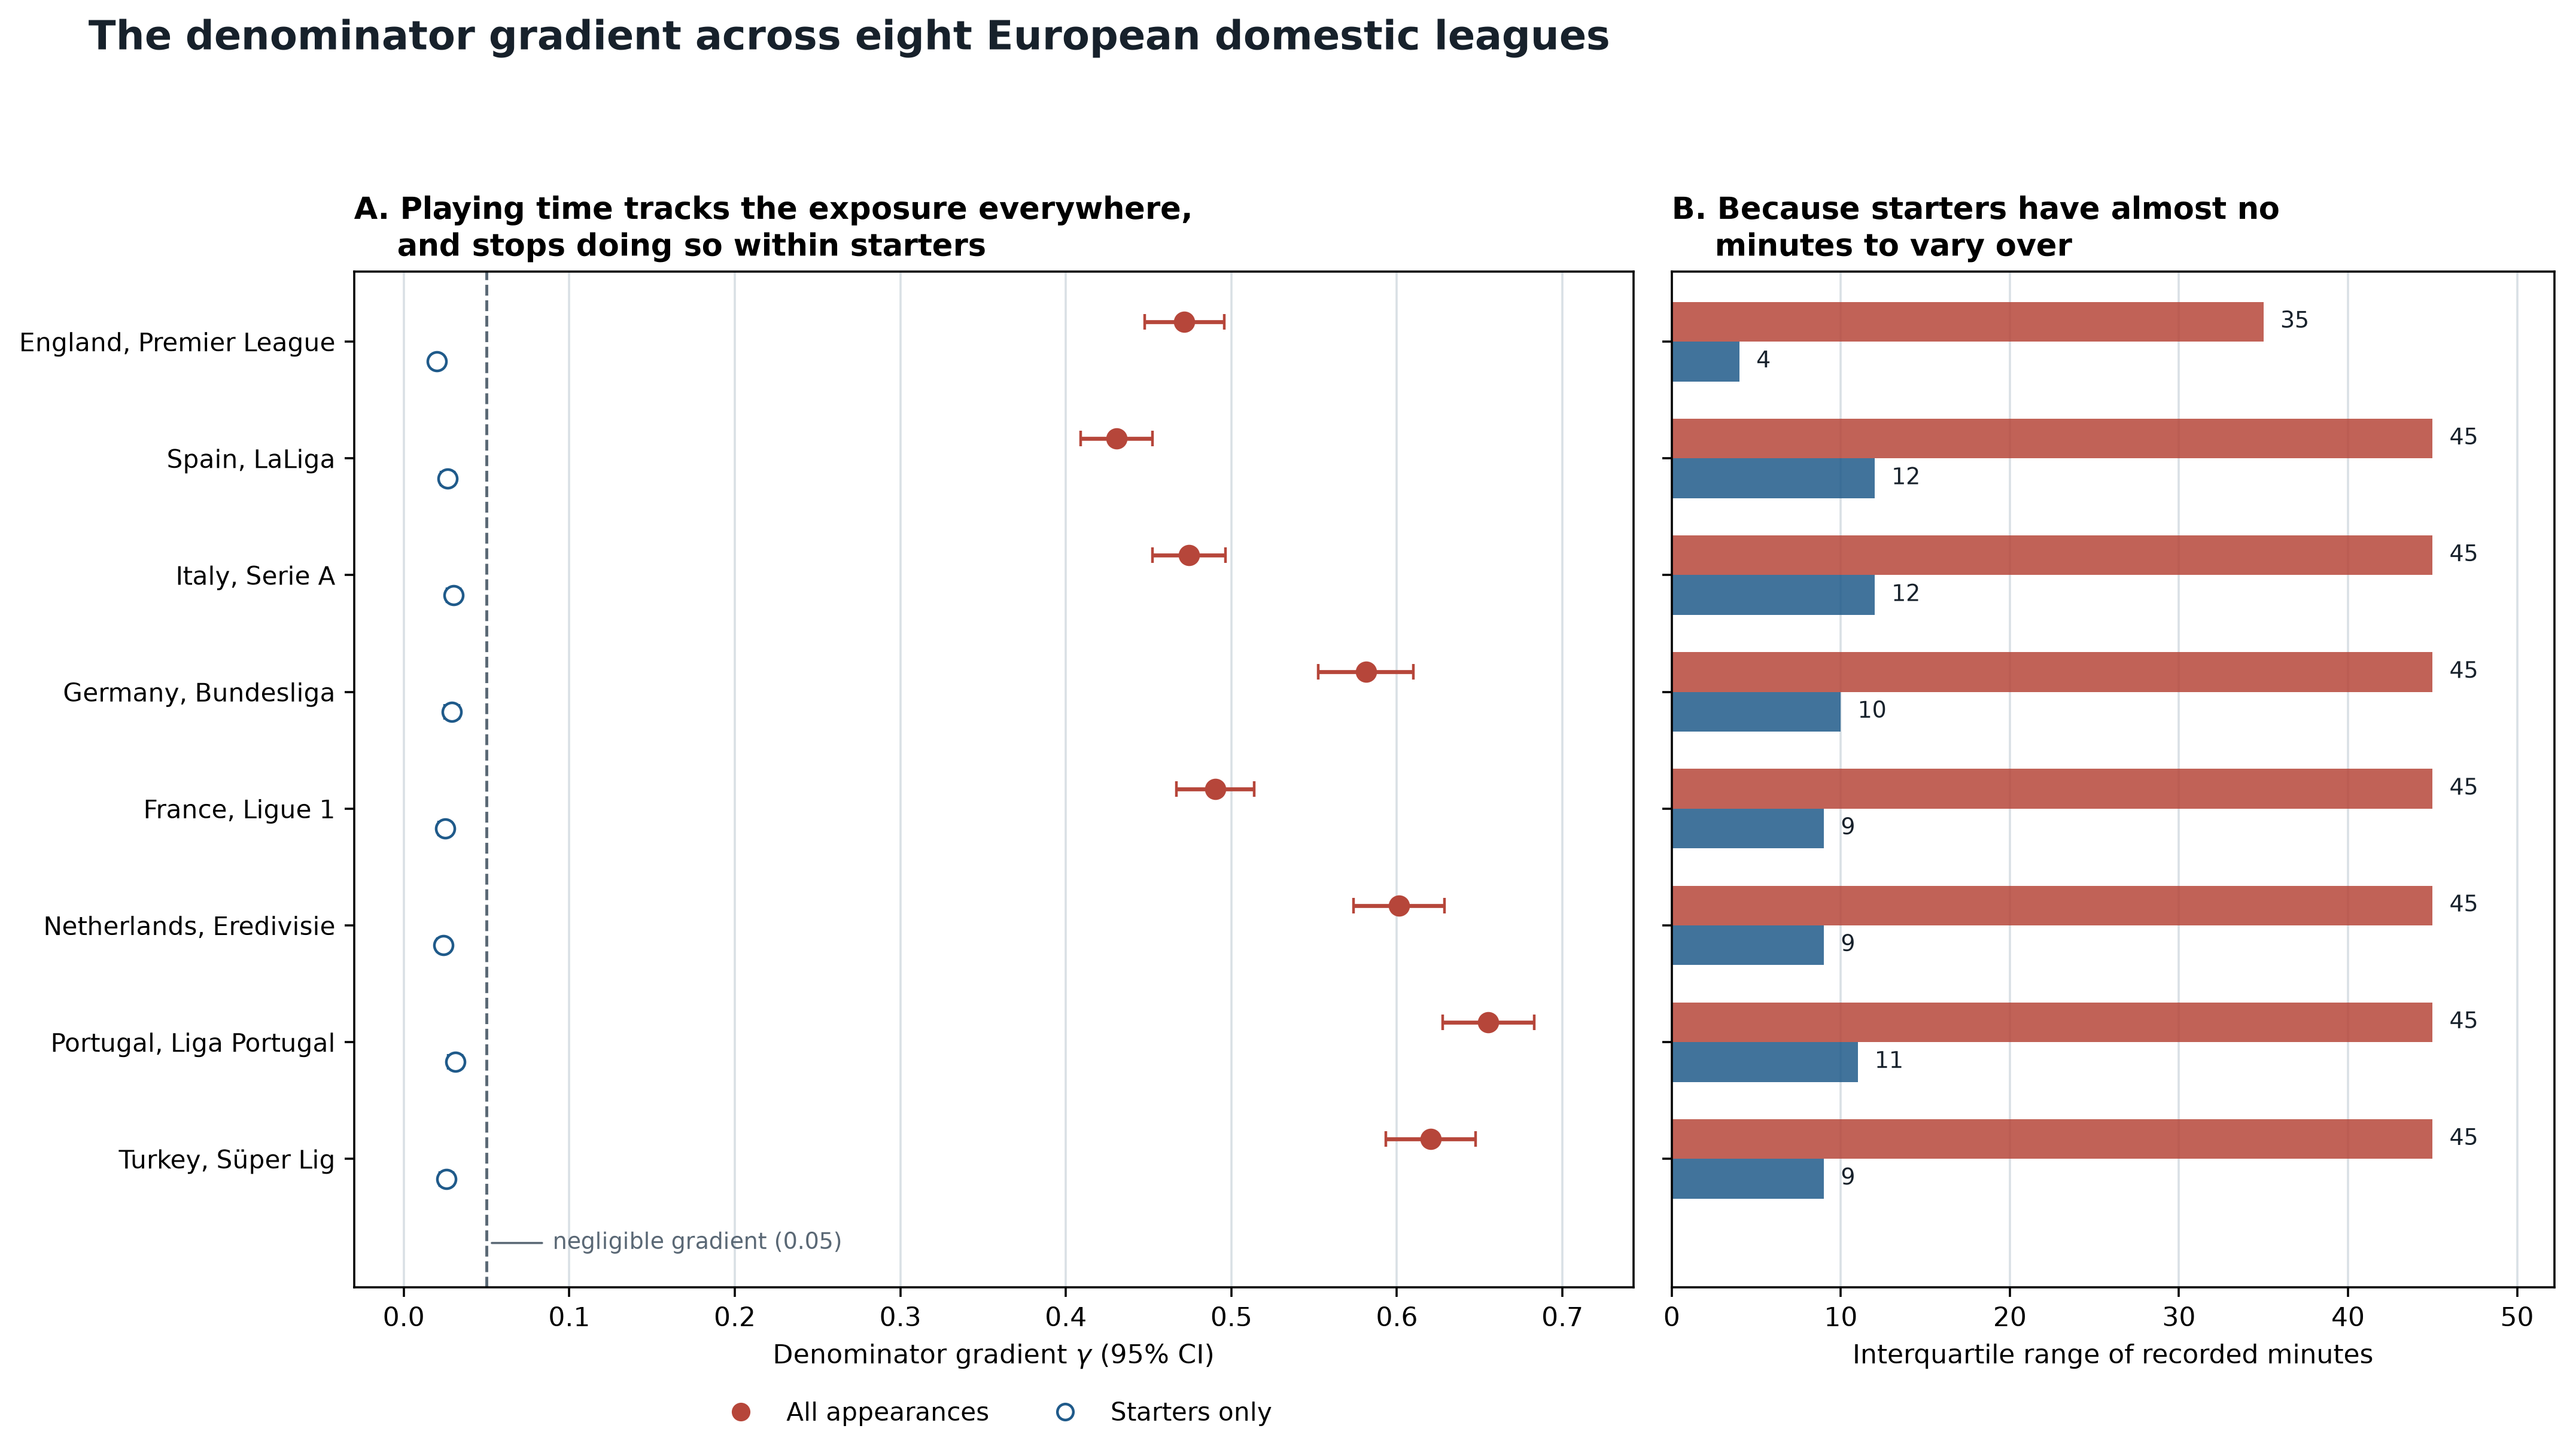
\includegraphics[width=\textwidth]{figures/J2_jsams_denominator_gradient.png}
\caption{The denominator gradient across the eight men's leagues, fitted from appearance records alone. Panel A gives $\gamma$ with player-clustered 95\% intervals, pooled and within starters, against the negligible threshold of 0.05. Panel B gives the interquartile range of recorded minutes in the same two populations and supplies the reason: an offset can only carry a gradient to the extent that it varies, and starters have almost no minutes to vary over.}
\label{fig:supp_gradient_men}
\end{figure}

\section{The gradient in women's leagues}

The men's panel comes from one provider and one sex, so on its own it cannot distinguish a property of squad rotation from a property of men's football or of one database. Women's competitions differ in country, squad size, fixture calendar, season geometry, sex and data provider simultaneously, which makes them the sharpest available test.

Women's appearances were read from Soccerdonna match reports, which publish each starting eleven and every substitution with its minute. Recorded minutes were therefore reconstructed rather than read: a starter plays until she is replaced, a substitute from the minute she enters, and a dismissal ends the appearance where it occurred. The reconstruction is checked on every match against the identity that twenty-two starters times ninety minutes totals 1980 recorded minutes, and a match failing that check is excluded rather than repaired. A league-season entered the panel only where the parsed reports covered at least 90\% of the league's own published fixture list.

\begin{table}[h]
\centering
\caption{The denominator gradient in seven women's European first tiers, one season each between 9 August 2024 and 16 November 2025. Fitted exactly as the men's gradients are, from appearance records alone with no injury data. Intervals are player-clustered. Coverage is the share of the league's published fixture list that produced a usable match report. The two rows whose within-starter interval reaches past the negligible threshold of 0.05 are the two where the decision rule returns risk per appearance rather than restriction to starters.}
\label{tab:supp_leagues_women}
\footnotesize
\setlength{\tabcolsep}{3pt}
\begin{tabular}{lrrrll}
\toprule
League & Appearances & Players & Coverage & Pooled $\gamma$ (95\% CI) & Within starters (95\% CI)\\
\midrule
England, FA Women's Super League & 3,924 & 297 & 132/132 & 0.466 (0.401--0.532) & 0.033 (0.019--0.047)\\
Germany, Frauen-Bundesliga & 3,999 & 304 & 132/132 & 0.456 (0.385--0.527) & 0.027 (0.010--0.043)\\
Spain, Primera División Femenina & 7,269 & 412 & 239/240 & 0.477 (0.420--0.535) & 0.038 (0.027--0.050)\\
Italy, Serie A Femminile & 2,737 & 245 & 90/90 & 0.494 (0.402--0.585) & 0.030 (0.011--0.049)\\
Norway, Toppserien & 3,937 & 247 & 135/135 & 0.444 (0.371--0.516) & 0.029 (0.018--0.041)\\
Sweden, Damallsvenskan & 5,278 & 345 & 181/182 & 0.647 (0.561--0.733) & 0.045 (0.032--0.058)\\
Switzerland, Women's Super League & 2,655 & 254 & 89/90 & 0.465 (0.383--0.547) & 0.027 (0.009--0.045)\\
\bottomrule
\end{tabular}
\end{table}

Three of the 1001 scheduled fixtures did not produce a usable match report, two to transient server errors and one to a report carrying only one lineup. All seven league-seasons cleared the coverage threshold, and every retained match satisfied the minute identity exactly.

\subsection*{Where the remedy stops working}

In five of the seven women's leagues the within-starter upper bound falls below the negligible threshold and the rule returns restriction to starters, as it does in all eight men's leagues. In Spain the bound reaches 0.050 and in Sweden 0.058, so the rule returns risk per appearance instead. We report this as an observed boundary rather than a finding about those two competitions. Each rests on a single season, the women's intervals are wider than the men's throughout because the panels are an order of magnitude smaller, and a wider interval alone can push an upper bound past a fixed threshold without the point estimate moving. What the exception demonstrates is that the rule discriminates: a remedy recommended everywhere without checking would have been wrong in two of the fifteen leagues measured here.

\section{Two providers, one league}

The women's panel and the men's panel come from different providers, which is a real threat to comparing them rather than a pedantic one. The Frauen-Bundesliga is the one competition covered by both providers used in this study, so the same league-season was fitted twice.

\begin{table}[h]
\centering
\caption{The Frauen-Bundesliga gradient fitted from two independent providers over the same season. Both fits use the same model, the same exposure window and the same player-clustered covariance; only the source of the appearance records differs.}
\label{tab:supp_cross_source}
\small
\begin{tabular}{lrl}
\toprule
Provider & Appearances & Pooled $\gamma$ (95\% CI)\\
\midrule
Soccerdonna match reports & 3,999 & 0.456 (0.385--0.527)\\
FBref match reports & 4,067 & 0.509 (0.429--0.588)\\
\bottomrule
\end{tabular}
\end{table}

The two differ by 0.053 with substantially overlapping intervals, and the two providers disagree slightly about how many appearances the season contained, which is itself informative about what a public appearance record is. Neither fit changes the verdict the rule returns. An overlap is not proof that two sources agree, but a non-overlap would have been proof that they do not, and would have made the men-and-women comparison unreportable.

\section{The public injury record in the two populations}

The main text restricts the outcome analysis to men's football and gives numbers rather than an assertion for why. Those numbers come from a matched audit: one sampling frame and one parser applied to the injury histories of current squads at eight women's and four men's clubs, 426 and 107 players respectively.

The audit measures three things, because three different failures would each disqualify the record as an outcome. \emph{Presence} is the share of sampled players carrying any recorded spell: 66.2\% against 86.0\%. \emph{Depth} is how far the record reaches back, measured per capita as the number of sampled players with a spell recorded in 2019--20 against the number with one recorded in 2024--25: 0.07 against 0.43. Because that comparison is made within the same players over time, it describes the recording rather than the injuries, and it is the finding that rules out a multi-season women's window. \emph{Severity mix} is the share of recorded spell descriptions naming a cruciate ligament injury: 9.9\% against 1.2\%. Nobody believes cruciate ruptures outnumber hamstring strains by that margin in either population, so the excess is a property of which injuries get reported.

Two cautions about the audit itself. Current squads are not a random sample of either population, although the frame is identical for both, so the comparison is fairer than either number alone. And part of the difference in spells per player follows from shorter women's seasons: a 22-match league produces fewer opportunities for injury than a 38-match one. That explanation does not touch the depth or severity comparisons, which is why those two carry the argument.

\section{Calibrating the identity, and what the threshold costs}

The first-order identity over-predicts the attenuation, and the size of the over-prediction is itself a function of the gradient. This section measures that function, and then translates a gradient into the quantity a reader actually reports.

The measurement comes first, because it is what the threshold is read against. Raising a floor on recorded minutes removes the short appearances, which is where most of the minute variation lives, so the gradient falls; the outcome, the exposure, the covariates and the clustering are unchanged. Table~\ref{tab:supp_curve} sweeps that floor across the whole range of the gradient, with a 95\% interval on each ratio from 1000 player resamples in which the entire sweep is recomputed. The unrestricted row reproduces both published quantities exactly, and the generator stops if it does not. An earlier version of this analysis had no sweep and filled the gap between the squad-role strata with the pooled ratio of 2.01, which is an extrapolation into the only part of the range the decision rule reads, and it ran in the direction that makes the threshold look about twice as tolerant as it is.

\begin{table}[h]
\centering
\caption{The over-prediction ratio measured across the range of the gradient. Each row restricts the cohort to appearances at or above a recorded-minute floor; nothing else about the model changes. Strata whose gradient interval includes zero are dropped, because a ratio of two quantities indistinguishable from zero is not a calibration. The final column is the percentile interval of the ratio over 1000 player resamples; it widens as the floor rises because fewer events survive. The floor-zero row is the published cohort.}
\label{tab:supp_curve}
\footnotesize
\setlength{\tabcolsep}{5pt}
\begin{tabular}{rrrrrrl}
\toprule
Minute floor & Appearances & Events & $\gamma$ & Attenuation & Ratio & Ratio 95\% CI\\
\midrule
82 & 54,670 & 89 & 0.001 & 0.001 & 0.94 & 0.46 to 4.20\\
75 & 58,920 & 124 & 0.004 & 0.004 & 0.96 & 0.80 to 1.23\\
65 & 64,341 & 183 & 0.009 & 0.010 & 0.96 & 0.87 to 1.06\\
55 & 67,932 & 238 & 0.015 & 0.016 & 0.97 & 0.91 to 1.04\\
40 & 71,460 & 376 & 0.024 & 0.023 & 1.06 & 1.00 to 1.12\\
20 & 78,108 & 496 & 0.078 & 0.057 & 1.36 & 1.29 to 1.43\\
0 & 88,573 & 576 & 0.303 & 0.151 & 2.01 & 1.92 to 2.12\\
\bottomrule
\end{tabular}
\end{table}

The ratio's point estimates rise monotonically, from 0.94 where the gradient is 0.001 to 2.01 where it is 0.303. The intervals temper what may be said about the small-gradient end: the point estimates sit within a few per cent of one there, and between $\gamma=0.004$ and $\gamma=0.024$ the intervals bear that out, with upper bounds no higher than 1.23; the very smallest floor, with 89 events, is too noisy to constrain the ratio at all (0.46 to 4.20), and is reported rather than leaned on. The region the threshold actually needs is well determined: at $\gamma=0.05$ the interval is 1.15 to 1.28. The factor of two is a large-gradient phenomenon, and the placebo exposure of a later section is consistent: it returns 1.99 at $\gamma=0.201$, against 1.36 (1.29 to 1.43) measured here at $\gamma=0.078$ and 2.01 (1.92 to 2.12) at $\gamma=0.303$.

Two scope notes. The curve is measured in this cohort, and the ratio is a property of the joint distribution of minutes, exposure and events rather than of $\gamma$ alone, so an analyst should sweep their own data rather than borrow these values; the sweep reuses the outcome model already being fitted, plus one least-squares fit per floor. That also marks its limit: unlike the gradient, the calibration needs an outcome, which is why it is reported for the reference cohort only --- the women's panels carry no injury data, so no second-population sweep is possible here.

Table~\ref{tab:supp_calibration} shows where the sweep came from: the four squad-role strata pair a gradient with the attenuation observed in the same rows, and the identity holds only within starters, where the gradient is small. The expansion weights every appearance equally while the Poisson score weights by fitted means, so the attenuation follows the minutes--exposure gradient among event-bearing rows rather than across the whole panel. Four strata leave a gap between $\gamma=0.011$ and $\gamma=0.214$ with the reporting threshold inside it, which is why the sweep exists.

\begin{table}[h]
\centering
\caption{The attenuation the first-order identity predicts against the attenuation observed, by squad-role stratum. The identity predicts an attenuation equal to $\gamma$. The final two columns express both as the percentage of the reported ratio that a recorded-minute denominator divides away, which is $1-\exp(-a)$ for an attenuation $a$.}
\label{tab:supp_calibration}
\footnotesize
\setlength{\tabcolsep}{5pt}
\begin{tabular}{lrrrrr}
\toprule
Stratum & $\gamma$ (predicted) & Observed & Ratio & Predicted \% & Observed \%\\
\midrule
All appearances & 0.303 & 0.151 & 2.01 & 26.2 & 14.0\\
Starters & 0.011 & 0.012 & 0.89 & 1.1 & 1.2\\
Substitutes & 0.214 & 0.117 & 1.84 & 19.3 & 11.0\\
Lineup unknown & 0.351 & 0.181 & 1.95 & 29.6 & 16.5\\
\bottomrule
\end{tabular}
\end{table}

The consequence for the reporting threshold is Table~\ref{tab:supp_threshold}. At $\gamma=0.05$ the measured ratio is 1.20 (1.15 to 1.28), so the threshold costs 4.1\% of the reported rate ratio, with a resampled interval of 3.8\% to 4.3\%: close to the 4.9\% the identity alone implies, and nothing like the 2.5\% a pooled ratio of 2.01 would have given. An analyst who wants the threshold to mean "no more than 5\% of my answer" should set it near 0.06. We keep 0.05, which is now shown to be a slightly conservative choice rather than the substantially over-conservative one the pooled calibration made it appear, and we report the translation so that the choice is visible and a different tolerance can be substituted.

\begin{table}[h]
\centering
\caption{What a gradient costs the reported rate ratio. The naive column reads the identity at face value; the calibrated column divides by the ratio measured at that gradient in Table~\ref{tab:supp_curve}. The final row lies beyond the swept range and its ratio is extrapolated, which is marked rather than hidden. The row in bold is the reporting threshold used throughout.}
\label{tab:supp_threshold}
\footnotesize
\setlength{\tabcolsep}{5pt}
\begin{tabular}{rrrrl}
\toprule
$\gamma$ & Ratio at this $\gamma$ & Naive \% & Calibrated \% & Ratio source\\
\midrule
0.010 & 0.96 & 1.0 & 1.0 & measured\\
0.025 & 1.07 & 2.5 & 2.3 & measured\\
\textbf{0.050} & \textbf{1.20} & \textbf{4.9} & \textbf{4.1} & measured\\
0.100 & 1.42 & 9.5 & 6.8 & measured\\
0.200 & 1.71 & 18.1 & 11.0 & measured\\
0.300 & 2.00 & 25.9 & 13.9 & measured\\
0.500 & 2.01 & 39.3 & 22.0 & extrapolated\\
\bottomrule
\end{tabular}
\end{table}

\section{Ascertainment across squad roles}

The remedy this paper recommends restricts the analysis to starters, so it is worth asking whether the public record observes starters and substitutes equally. It does not observe them equally per appearance: a same-day report attaches to 6.7 per 1000 starter appearances against 2.0 per 1000 substitute appearances (Wilson intervals 6.1--7.5 and 1.3--2.9), a ratio of 3.46.

That gap is exposure, not reporting. A starter records a mean of 84.9 minutes and a substitute 20.0, and per 1000 recorded minutes the ordering inverts: 0.079 among starters against 0.097 among substitutes, a ratio of 0.82. If the record were systematically missing substitutes' events --- a plausible worry, since a player withdrawn after twenty minutes attracts less coverage than one carried off after seventy --- the per-minute rate among substitutes would be the lower of the two. It is the higher. Rows with no lineup status sit above both, at 8.8 per 1000 appearances and 0.130 per 1000 minutes. We do not offer an explanation for that: thin lineup coverage would account for the missing status but not for a higher event rate, and we have no way to separate the possibilities with these data.

This does not prove that reporting is unbiased; it rules out the specific direction that would make restriction to starters self-defeating. A misclassification acting equally on both roles would be invisible to this comparison, and is admitted as such in the main text.

\section{Clustering the covariance three ways}

Every interval in this paper is clustered on player identifier, because appearances repeat within player. They also repeat within club-season, and squad rotation is a club decision rather than a player one, and they repeat within fixture. Table~\ref{tab:supp_clustering} refits the reference gradient under each.

Nothing about the estimate can move, and nothing does: clustering is a choice of covariance, not of estimator, so the three rows carry an identical gradient. The generator checks this rather than assuming it, and stops the run if the baseline row fails to reproduce the published value --- a first attempt at this table silently dropped the history term the published model conditions on and returned 0.321, which would have been reported as a clustering effect when it was a different model.

\begin{table}[h]
\centering
\caption{The reference gradient under three clusterings. The estimate is identical by construction; only the interval moves. Fixture clustering gives the narrowest interval because a fixture contains at most twenty-two of the cohort's appearances, and club-season the widest because a club-season contains hundreds.}
\label{tab:supp_clustering}
\footnotesize
\setlength{\tabcolsep}{6pt}
\begin{tabular}{lrrrl}
\toprule
Clustering & Groups & $\gamma$ & Std.\ error & 95\% CI\\
\midrule
Player (published) & 1,208 & 0.303 & 0.0101 & 0.283 to 0.323\\
Club-season & 201 & 0.303 & 0.0108 & 0.282 to 0.324\\
Fixture & 6,902 & 0.303 & 0.0062 & 0.291 to 0.315\\
\bottomrule
\end{tabular}
\end{table}

The widest interval is 1.74 times the narrowest, and every lower bound sits above 0.28. The published clustering is neither the most nor the least conservative of the three, and no verdict in this paper changes under any of them. Fixture is arguably the wrong level: a fixture contains two clubs whose rotation decisions are made independently, so clustering there groups appearances that share a date rather than a decision. We report it because it is the narrowest of the three and therefore the least favourable to a claim of robustness, not because we think it is the correct unit.

\section{The precision the panels delivered}

No target sample size was set, because the panel is every admitted appearance in the selected competitions rather than a recruited sample. The honest substitute for a power statement is the precision actually achieved. Across the eight men's leagues the half-width of the pooled gradient's interval ran from 0.022 to 0.029, between 4.2\% and 5.1\% of the estimate. Across the seven women's leagues, which are one season each and between ten and thirty times smaller, it ran from 0.057 to 0.092, between 12.0\% and 18.5\% of the estimate. The least precise panel is Italy's Serie A Femminile at 2,737 appearances, whose interval is 0.402 to 0.585: wide, and still an order of magnitude clear of the 0.05 threshold. Every pooled verdict in this paper is therefore carried by an interval that does not come close to the threshold it is read against. The within-starter verdicts are the tighter question, and the two leagues where they fall the other way are reported as such in the main text.

\section{The identity replicated on a placebo exposure}

The first-order identity predicts an attenuation of $\gamma$ and delivers about half of it, because the expansion weights appearances equally whereas the Poisson score weights by fitted means. If that ratio were a property of the seven-day exposure it would be a coincidence worth worrying about. It is not.

\begin{table}[h]
\centering
\caption{The denominator decomposition repeated on the placebo exposure, minutes played 31--37 days earlier, which has no plausible causal path to a same-day report. All fits use the same 88,573 rows and 576 events as the reference analysis, with player-clustered intervals.}
\label{tab:supp_placebo_denominator}
\small
\begin{tabular}{lll}
\toprule
Quantity & Placebo window & Reference exposure\\
\midrule
Per appearance & 1.147 (1.011--1.301) & 1.267 (1.112--1.445)\\
Fixed 90 minutes & 1.146 (1.011--1.299) & 1.265 (1.111--1.441)\\
Recorded minutes & 1.036 (0.913--1.175) & 1.088 (0.951--1.245)\\
Denominator gradient $\gamma$ & 0.201 (0.187--0.216) & 0.303 (0.283--0.323)\\
Observed attenuation & 0.101 & 0.151 (0.140--0.163)\\
$\gamma$ over observed attenuation & 1.99 & 2.01\\
\bottomrule
\end{tabular}
\end{table}

The placebo carries a smaller gradient and a correspondingly smaller attenuation, and the ratio between what the identity predicts and what is observed is 1.99 against 2.01. Two exposures chosen for different reasons, one of which should have no causal path at all, produce the same structural over-prediction. That is what one expects if the arithmetic is a property of the denominator rather than of the exposure, and it is why the main text rests the attribution on the direct offset comparison rather than on $\gamma$.

Note also what the placebo does not do. Its per-appearance estimate is 1.147 (1.011--1.301), which excludes one; the placebo window is not a clean null, and the main text says so. Reporting propensity is present and only partly separable from recent load. That limits what the placebo can rule out about the worked example, but it does not limit what it demonstrates about the denominator, which is a claim about arithmetic on shared rows.

\section{Reproducibility files}

The central revised files share the prefix \path{jsams_revised_}:
\begingroup
\small
% Filenames are single unbreakable tokens, so the default line-breaking
% tolerance pushes them past the text block. Loosening it inside this list
% only stretches the spaces between them.
\sloppy
\begin{itemize}
  \item exposure results: \path{exposure_multiverse.csv}, \path{additive_curves.csv} and \path{temporal_stability.csv};
  \item conditional results: \path{conditional_estimates.csv} and \path{conditional_population.csv};
  \item selection results: \path{appearance_selection_estimates.csv} and \path{appearance_selection_diagnostics.csv};
  \item denominator mechanism: \path{recorded_minute_distribution.csv}, \path{lineup_composition_by_exposure.csv}, \path{denominator_by_lineup_role.csv}, \path{denominator_attenuation_decomposition.csv}, \path{direct_truncation_refit.csv}, \path{attenuation_bootstrap.csv}, \path{case_restricted_exposure_bias.csv}, \path{truncation_imputation_sensitivity.csv}, \path{squad_role_association_sensitivity.csv}, \path{role_adjusted_denominator_refit.csv}, \path{exposure_window_gradient.csv}, \path{run_in_exclusion_comparison.csv}, \path{placebo_denominator_replication.csv}, \path{denominator_gradient_by_league.csv}, \path{denominator_gradient_decision_rule.csv}, \path{denominator_gradient_summary.csv}, \path{denominator_gradient_clip_sensitivity.csv}, \path{denominator_gradient_estimator_sensitivity.csv}, \path{denominator_gradient_specifications.csv} and \path{lineup_coverage_denominator_stability.csv};
  \item cohort description: \path{event_clustering_summary.csv}, \path{model_field_completeness.csv} and \path{episode_type_composition.csv};
  \item robustness: \path{confounding_sensitivity.csv}, \path{club_congestion_sensitivity.csv}, \path{run_in_threshold_sensitivity.csv} and \path{exposure_metric_correlations.csv};
  \item negative controls and ascertainment: \path{placebo_window_analysis.csv}, \path{negative_control_outcomes.csv} and \path{ascertainment_by_exposure.csv};
  \item audit and reporting records: \path{outcome_audit_summary.csv}, \path{outcome_audit_validation.csv}, \path{non_event_audit_queue.csv}, \path{non_event_absence_screen.csv}, \path{non_event_audit_summary.csv}, \path{missed_event_adjudication_protocol.csv}, \path{second_assessor_agreement.csv}, \path{claim_hierarchy.csv} and \path{hypothesis_register.csv};
  \item scoping search: \path{per_minute_denominator_scoping.csv} and \path{per_minute_denominator_scoping_protocol.csv}.
\end{itemize}
\endgroup
The opportunity-resolution audit is \path{selection_membership_resolution_audit.csv}. Three hand-built files no script can regenerate are preserved under \path{data/manual/}: \path{independent_same_day_event_audit.csv}, the exposure-blinded same-day outcome audit; \path{independent_non_event_audit.csv}, the report-free queue review with its per-record notes; and \path{per_minute_denominator_scoping.csv}, the scoping records with the verbatim sentence behind every confirmed denominator. Daily models, crude plots, FFT diagnostics and earlier category analyses remain in the versioned archive but are not main-paper evidence.

Analyses used Python 3.12.10 with pandas 2.3.3, numpy 2.3.5, statsmodels 0.14.5, patsy 1.0.2, scipy 1.16.3 and matplotlib for figures. Script \path{src/36_jsams_second_referee_analysis.py} fits every model and writes 50 \path{jsams_revised_*} tables under a fixed random seed; \path{src/37_denominator_gradient.py} writes a further nine, including the cross-league gradients, the decision rule, the estimator and floor sensitivities, the specification register and both deposited protocols. The women's panel is assembled by \path{src/39_fetch_fbref_womens_appearances.py}, which validates every match report before admitting it and replaces source player identifiers with surrogates drawn at random; \path{src/40_womens_denominator_gradient.py} fits the women's gradients by calling script 37's estimator unchanged, so a difference between the populations cannot come from two versions of one regression; and \path{src/41_womens_injury_record_audit.py} turns the injury-record audit into the aggregates reported here, none of which name anybody. Script \path{src/42_statistical_output_appendix.py} refits all 30 reported gradients, checks each against the deposited estimate and stops on any mismatch, then writes the full statistical output supplied as Appendix A. Script \path{src/35_plot_jsams_revision.py} reads the deposited tables and writes nine figures --- five shown in the main paper and four here --- without refitting anything. Script \path{src/44_referee_response_analysis.py} computes the quantities added in revision: the calibration of the first-order identity against the attenuation actually observed, the translation of a gradient into the percentage of the association it removes, the ascertainment comparison across squad roles, the clustering sensitivity, and the precision each league panel delivered. Script \path{src/43_strobe_checklist.py} generates the STROBE checklist in Section~1, resolving each item against the manuscript source and stopping rather than emitting an item that points at text the manuscript does not contain.

\begingroup
\footnotesize
\bibliography{references}
\endgroup

\end{document}
